\chapter{Cell assembly analysis}
\label{chap:AssemblyAnalysis}
In this chapter I present the assembly analysis conducted on the data set introduced in \hyperref[sec:Dataset]{Section~\ref*{sec:Dataset}}, using the cell assembly detection algorithm and the single units classification presented in \hyperref[chap:AssemblyMethod]{Chapter~\ref*{chap:AssemblyMethod}} and \hyperref[chap:UnitsAnalysis]{Chapter~\ref*{chap:UnitsAnalysis}} respectively.\\
The cell assembly detection algorithm is designed to detect any coordinated spike trains patterns at any time scale. The time scales were explored by binning the spike train with different bin-widths. Further I examined the lag distribution. Lags describe the temporal distance in activations between units in the assembly. Applying the cell-assembly algorithm I detected synchronous ($lag=0$) and asynchronous ($lag\neq0$) cell assemblies at arbitrary time scale ($\Delta$).\\Being interested in cross areal interactions and directionality between ventral striatum (VS) and ventral tegmental area (VTA), I focused the study on interregional assembly-pairs, that are formed by two neurons, of which one neuron is located in the VS and the other one in VTA. A positive lag ($lag>0$) indicates that the activatio of the VS unit precedes the activation of the VTA unit, or in other words: VS is leading and VTA is following. A negative lag ($lag<0$) means that the activation of VTA unit is preceding the activation of the VS unit, hence VTA is leading and VS is following.\\\\\\\\\\\\\\\\\\\\\\\\\\\\\\
\section{Cell types occurrence}
\label{sec:AsseTypes}
Based on the unit classification (\hyperref[chap:UnitsAnalysis]{Chapter~ \ref*{chap:UnitsAnalysis}}), interregional assembly were divided according to their underlying cell-types (figure \ref{fig:PieAssembliesTot} (B.)).
\begin{figure}[H]
    \centering
    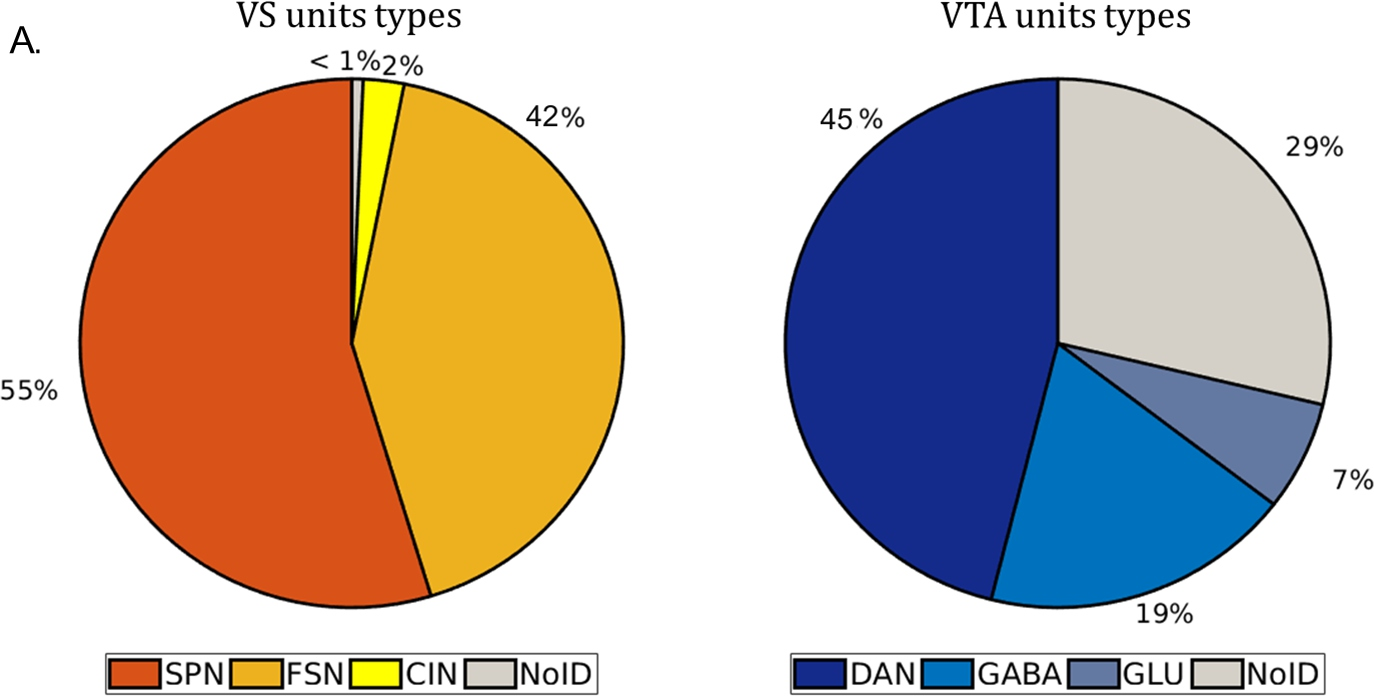
\includegraphics[scale=0.4]{figures/PieRegions2.pdf}
    
    \vspace{0.5 cm}
    
    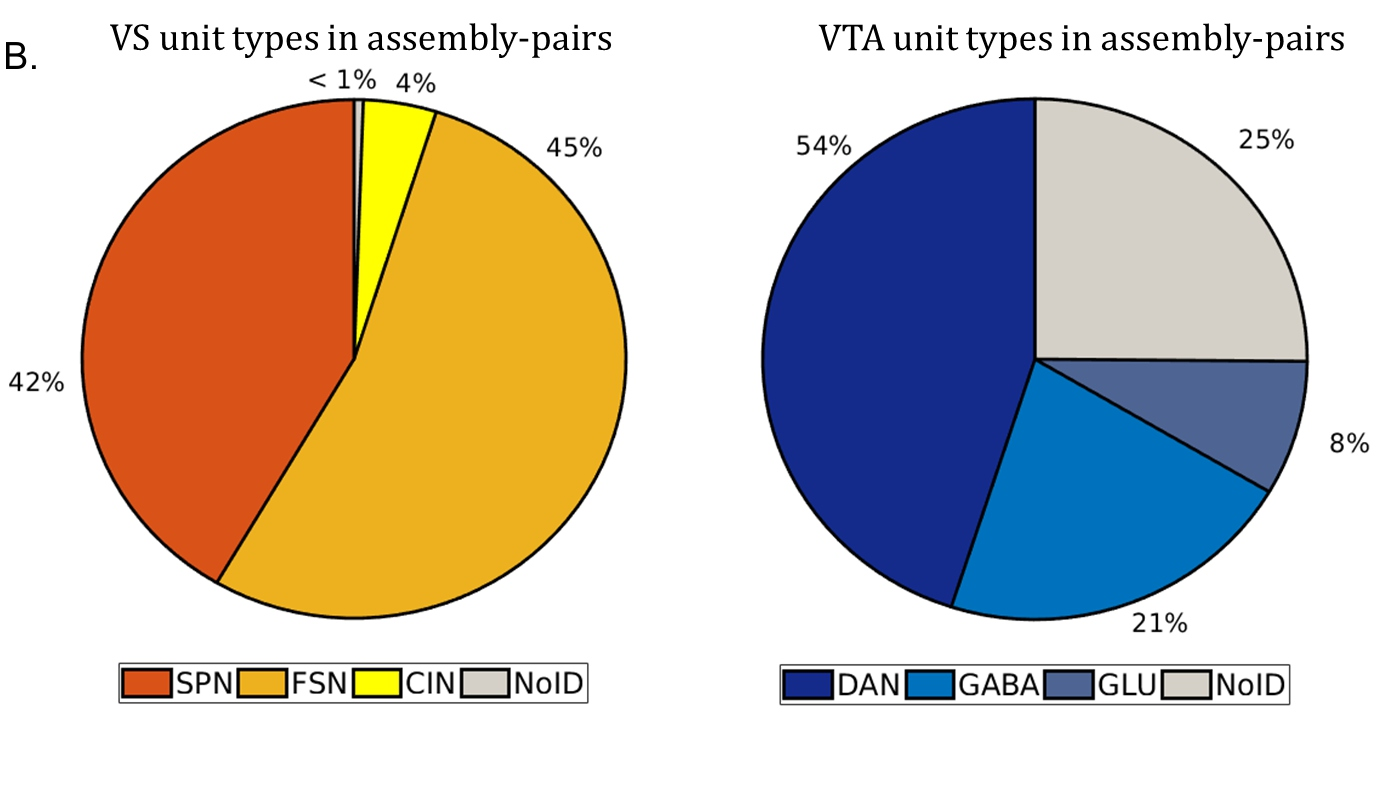
\includegraphics[scale=0.4]{figures/PieAsNotAs.pdf}
    
    \vspace{0.5 cm}
    
    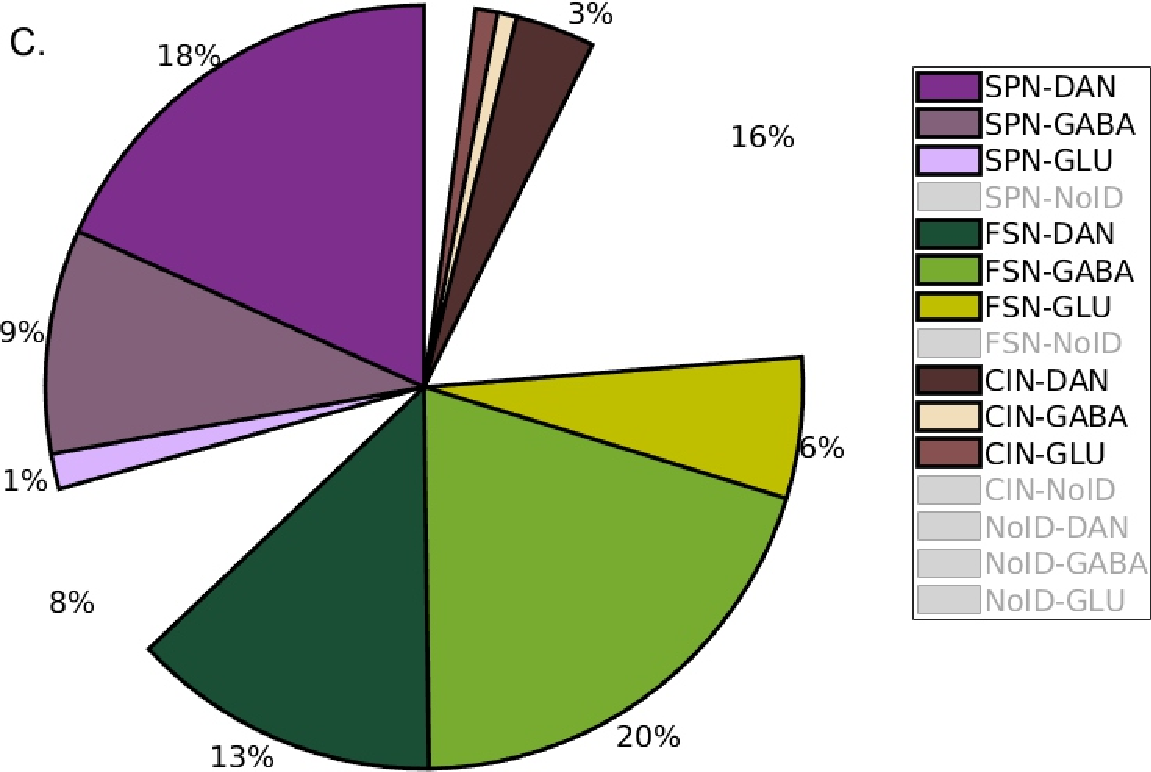
\includegraphics[scale=0.4]{figures/PieAssembliesTot1.pdf}
    \caption{(A.) Occurrence of classified and non-classified units in VS and VTA. (B.) Occurrence of classified and non-classified units of VS and VTA in interregional assembly-pairs. In VS, FSN occur in interregional pairs more often than SPN, even though more SPN than FSN were recorded. (C.) Pie charts of assemblies types. Cell types with $<1\%$ are not indicated. Missing pieces of cake indicates pairs that include non-classified units. The four more frequent interregional pairs, including only classified units, are pairs between fast spiking and gabaergic neurons ($20\%$), striatal projection neurons and dopamine neurons ($18\%$), fast spiking and dopamine units ($13\%$), and striatal projection and gabaergic units ($9\%$). }
    \label{fig:PieAssembliesTot}
\end{figure}
Comparing the two pie charts related to the VS region (figure \ref{fig:PieAssembliesTot} (A. vs B.)), one observes that FSN occurred in interregional pairs more often than SPN (figure \ref{fig:PieAssembliesTot} (B.,left)), even though in the total sample of recorded neurons FSN are less frequent than SPN (figure \ref{fig:PieAssembliesTot} (A.,left)).
\label{sec:CellTypesOcc}
I hypothesized that specific cell-types had a higher tendency to aggregate into cell assemblies. To verify this hypothesis, I conducted for each of the two regions a Pearson's $\chi^2$ test. Of the classified unit types, only those with sufficient cell count could be tested for reasons of statistical power: namely SPN and FSN in VS, and DAN and GABA units in VTA. I therefore focused on the four most prominent neuron types and the cell assembly pairs formed between those units.
\begin{table}[H]
    %\centering
\begin{tabular}{ |p{3cm}|p{3cm}|p{3cm}| }
 \hline
 \multicolumn{3}{|c|}{Pearson$'$s $\chi^2$ test VS unit type and interregional pair relationship} \\
 \hline
 & In assemblies & Not in aseemblies\\
 \hline
 SPN & 153 (197.64) & 253 (208.36) \\
 \hline
 FSN & 197 (156.36) & 116 (164.64)\\
 \hline
 \multicolumn{3}{|c|}{$\chi^2$ statistic  45.13}\\
 \multicolumn{3}{|c|}{p-value = $1.8\times10^{-11}$}\\
 \hline
 \multicolumn{3}{|c|}{$\chi^2$ statistic Yates correction 44.12}\\
 \multicolumn{3}{|c|}{p-value = $3.1\times10^{-11}$}\\
 \hline
\end{tabular}
\caption{Pearson's $\chi^2$ contingency table with $\chi^2$ value and p-value. Unit-types and interregional pairs formation are correlated in VS.}
\label{tab:chi2_asnotasVS}
\end{table}
\begin{table}[H]
    %\centering
\begin{tabular}{ |p{3cm}|p{3cm}|p{3cm}| }
 \hline
 \multicolumn{3}{|c|}{Pearson's $\chi^2$ test VTA unit-type and interregional pair relationship} \\
 \hline
 & In assemblies & Not in aseemblies\\
 \hline
 DAN & 86 (90.604) & 31 (26.40) \\
 \hline
 GABA & 41 (36.40) & 6 (10.60)\\
 \hline
 \multicolumn{3}{|c|}{$\chi^2$ statistic  3.62}\\
 \multicolumn{3}{|c|}{p-value = 0.057}\\
 \hline
\end{tabular}
\caption{Pearson's $\chi^2$ contingency table with $\chi^2$ value and p-value. Unit-types and interregional pairs formation are not correlated in VTA.}
\label{tab:chi2_asnotasVTA}
\end{table}
Whether the recorded unit may or may not be part of an interregional pair is described  in the contingency tables \ref{tab:chi2_asnotasVS}, \ref{tab:chi2_asnotasVTA}. In the contingency tables, the number (compared to the expected values indicated in parentheses) of specific cell types in interregional pairs were reported with $\chi^2$ statistic p-values. For each test the $\alpha$ significance level was fixed at $0.05$, unless otherwise specified.\\A relationship between unit types and interregional pairs formation was found only in VS. In VS the $\chi^2$ statistic value is 45.13 (44.12 using Yates correction), that gives a p-value of $1.8\times10^{-11}$ ($3.1\times10^{-11}$) (\ref{tab:chi2_asnotasVS}). The results confirmed that in VS the tendency of being agglomerate in interregional pairs depended on the specific cell-type. Specifically, FSN result more prone to participate to interregional assemblies. A similar test was conducted in VTA, with a resulting $\chi^2$ statistic of $3.62$ and a p-value of $0.057$, not significant at $\alpha = 0.05$ level (\ref{tab:chi2_asnotasVTA}). I therefore conclude that in VTA different cell-types had more comparable probabilities to agglomerate in interregional pairs.\\I have shown above how often VS and VTA units occur in assemblies. I next analyzed if specific interregional pair-types occur systematically more often than others. The occurrence of assembly-types for the recorded units is shown in the pie-chart of figure \ref{fig:PieAssembliesTot} (bottom). Selecting only classified units, four assembly types occurred more often than others, they were pairs formed by FSN and GABA (20$\%$), SPN and DAN (18$\%$), FSN and DAN (13$\%$) and SPN and GABA (9$\%$).\\To see whether there was a preferential pairing specific unit types in forming interregional assemblies, also in relation to the assembly directionality, I performed a Pearson$'$s $\chi^2$ test on the four more frequent assembly group. Specifically, given the relative frequency of certain types of assemblies, I hypothesized a preference for fast spiking neurons with gabaergic neurons (and/or vice-versa) and a preference for striatal projection neurons with dopamine neurons (and/or vice-versa).
\begin{table}[H]
    %\centering
\begin{tabular}{ |p{3cm}|p{3cm}|p{3cm}| }
 \hline
 \multicolumn{3}{|c|}{Pearson's $\chi^2$ test ($VS \rightarrow VTA$)} \\
 \hline
 & DAN pairs & GABA pairs\\
 \hline
 SPN & 76 (63.77) & 35 (47.23) \\
 \hline
 FSN & 32 (44.23) & 45 (32.77)\\
 \hline
 \multicolumn{3}{|c|}{$\chi^2$ statistic  13.47}\\
 \multicolumn{3}{|c|}{p-value = $2\times10^{-4}$}\\
 \hline
 \multicolumn{3}{|c|}{$\chi^2$ statistic Yates correction 12.39}\\
 \multicolumn{3}{|c|}{p-value = $4\times10^{-4}$}\\
 \hline
\end{tabular}
\caption{Pearson's $\chi^{2}$ test contingency table. I tested the dependency between the neuron type in VS and the neuron type in VTA, for pairs with specific directionality $VS \rightarrow VTA$. The $\chi^2$ test show a dependency among variables, meaning that specific pairs have higher tendency to agglomerate in assembly.}
\label{tab:chisquare_vsvta}
\end{table}
\begin{table}[H]
\begin{tabular}{ |p{3cm}|p{3cm}|p{3cm}| }
 \hline
 \multicolumn{3}{|c|}{Pearson$'$s $\chi^2$ test ($VS \leftarrow VTA$)} \\
 \hline
 & SPN pairs & FSN pairs\\
 \hline
 DAN & 18 (12.06) & 29 (34.94) \\
 \hline
 GABA & 11 (16.94) & 55 (49.06)\\
 \hline
 \multicolumn{3}{|c|}{$\chi^2$ statistic  6.73}\\
 \multicolumn{3}{|c|}{p-value = 0.009}\\
 \hline
 \multicolumn{3}{|c|}{$\chi^2$ statistic Yates correction 5.65}\\
 \multicolumn{3}{|c|}{p-value = 0.017}\\
 \hline
\end{tabular}
\caption{Pearson$'$s $\chi^{2}$ test contingency table. I tested the dependency between the neuron type in VTA and the neuron type in VS, for pairs with specific directionality $VS \leftarrow VTA$. The $\chi^2$ test show a dependency among variables, meaning that specific pairs have higher tendency to agglomerate in assembly.}
\label{tab:chisquare_vtavs}
\end{table}
The $\chi^2$ test was performed on the directional pairs ($lag\neq0$) and separately on $VS\rightarrow VTA$ ($lag>0$) and $VS\leftarrow VTA$ ($lag<0$). In both cases, the p-values of $\chi^2$ test were significant at the confidence level $\alpha = 0.05$, hence the confirming a dependence between the cell-type and the resulting interregional assembly pair type. In direction $VS\rightarrow VTA$ the p-value was $2\times10^{-4}$ ($p=4\times10^{-4}$ using Yates correction), in direction $VS\leftarrow VTA$: $p=9\times10^{-3}$ ($p=0.017$ using Yates correction). The contingency and the results of the $\chi^2$ tests are shown for the two directionalities in tables \ref{tab:chisquare_vsvta} and \ref{tab:chisquare_vtavs}. Both in $VS\rightarrow VTA$ and in $VS\leftarrow VTA$ directionalities the occurrence of the couples $SPN+DAN$ and $FSN+GABA$ exceed the values expected in case of independence.
\section{Inter-/intra- regional pair time scales}
\label{sec:TimeScales}
In the previous session I have seen that in VS the neuronal occurrence in assembly depends on the cell-types, and that specifically FSN occur more frequently in assembly than SPN. Furthermore I have seen that, in directional assemblies, the combination among cell types is non-random. With these analysis I described the cell types occurrence in VS-VTA interactions. Time scales involved in the cross-area interactions will be examined later in this chapter, together with a comparison with intra-area interaction time scales.\\As introduced in \hyperref[chap:AssemblyMethod]{~Chapter \ref*{chap:AssemblyMethod}}, the assembly detection method CAD is able to detect cell-assemblies within a range of temporal precision $\Delta\in\{\Delta_{min},...,\Delta_{max}\}$ provided by the user. Pairs were tested at all possible bin widths, then for each assembly, the width $\Delta^*$ associated with the lowest p-value was chosen as its characteristic temporal precision (\cite{RussoDurstewitz}, see \hyperref[chap:AssemblyMethod]{Chapter~ \ref*{chap:AssemblyMethod}}).\\For the following analysis I focused the assembly search on temporal precision ranging from 0.01 s to 0.6 s. Figure \ref{fig:BinDistr} shows the temporal scale ($\Delta$) distribution of VS-VTA interregional-interactions. Figures \ref{fig:BinDistrVS} and \ref{fig:BinDistrVTA} show VS-VS and VTA-VTA time-scale interactions distribution respectively.\\A comparison among interregional pairs (VS-VTA pairs) and intraregional pairs (VS-VS pairs and VTA-VTA pairs) showed interesting differences: while I observed assemblies with temporal precision at the scale of few tens of milliseconds only within either VS or VTA, assemblies of lower temporal precision were detected across VS-VTA units. Interregional VS-VTA interactions had a bimodal time-scales distribution with two peaks, one around 80 $ms$ and one around 0.6 $sec$, revealing two time scales involved in VS-VTA interaction. The first, more precise time scale, ranged from 10 $ms$ to 250 $ms$, and the second included broader bin sizes.\\Bimodality was a characteristic specific of VS-VTA interactions, not present neither in VTA-VTA, nor in VS-VS interactions: intraregional VTA-VTA pairs did not present any peak in time scale distribution, whereas intraregional VS-VS bin size distribution peaked around 50 $ms$.  
\begin{figure}[H]
\centering
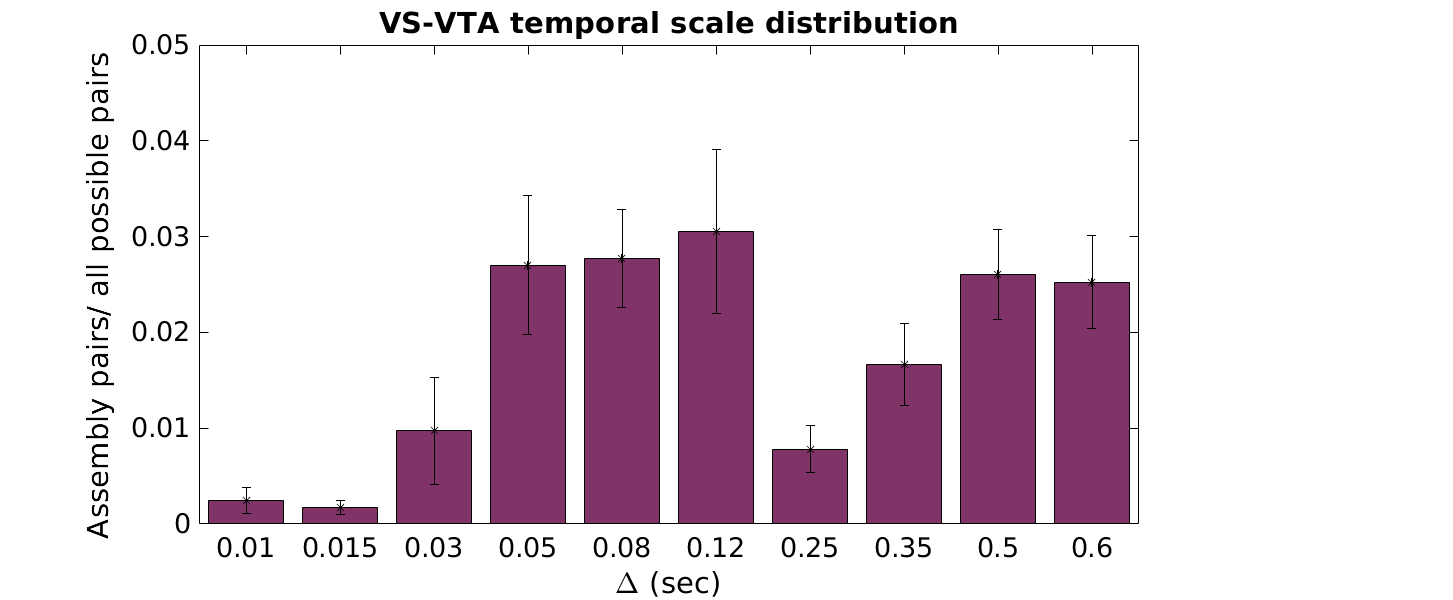
\includegraphics[scale=0.48]{figures/VS_VTA_Short1.png}
\caption{Bin distribution for interregional pairs. VS-VTA pairs show a bimodal distribution, revealing two temporal scales involved in interregional activation patterns.}
\label{fig:BinDistr}
\end{figure}
\begin{figure}[H]
\centering
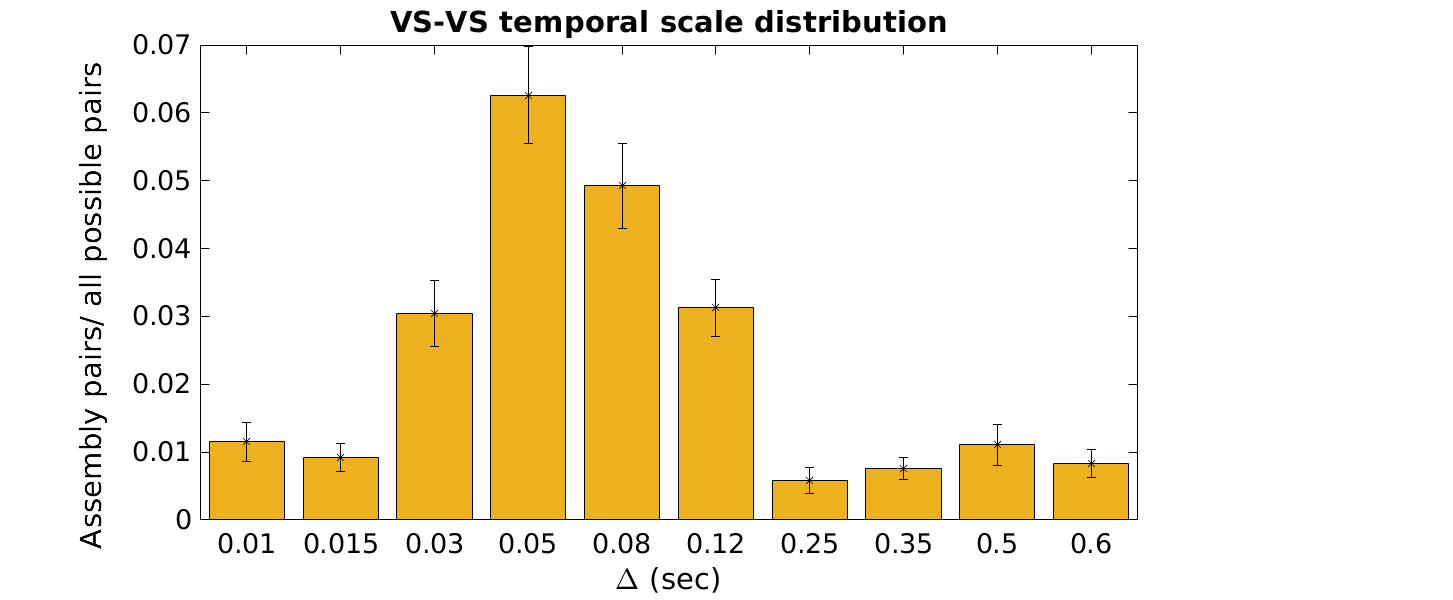
\includegraphics[scale=0.48]{figures/VS_VS_S.png}
\caption{VS-VS pairs are more precise than VS-VTA pairs and the bin distribution presented with a peak at 50 $ms$}
\label{fig:BinDistrVS}
\end{figure}
\begin{figure}[H]
\centering
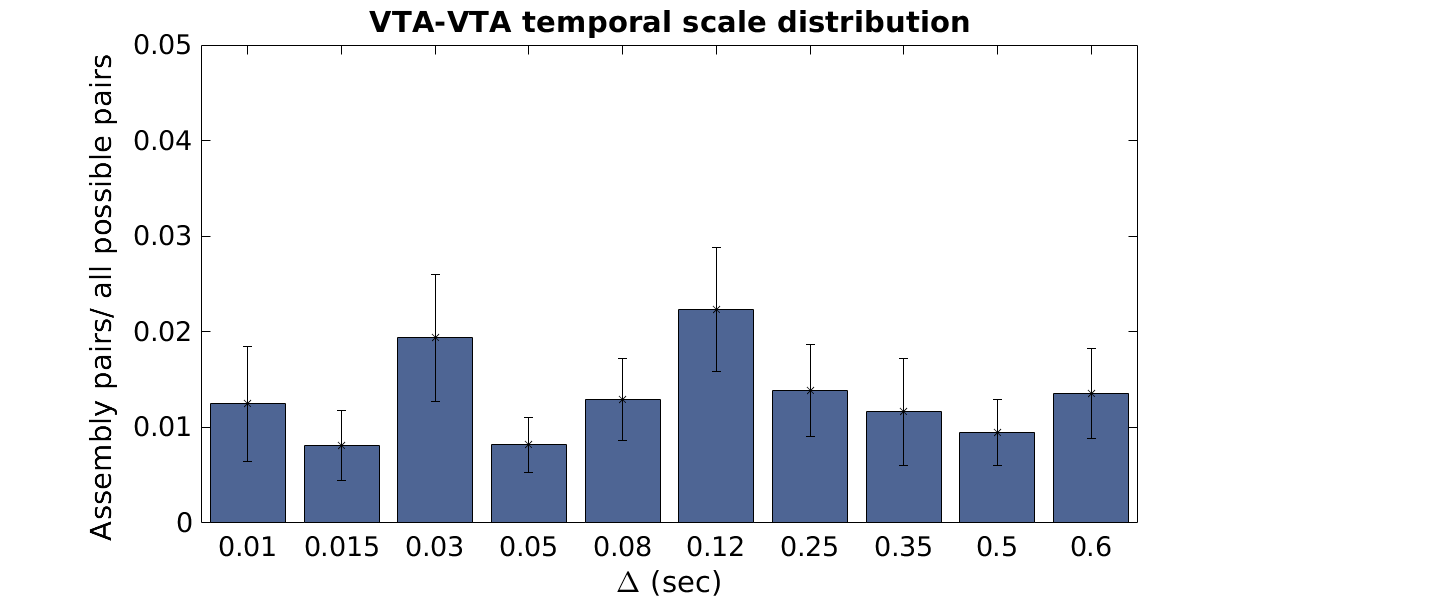
\includegraphics[scale=0.48]{figures/VTA_VTA_S.png}
\caption{VTA-VTA temporal scales were broadly distributed.}
\label{fig:BinDistrVTA}
\end{figure}
\subsection{SPN-FSN time scales interactions}
\label{sec:SPN-FSN_Bin}
FSN have a broad range of baseline firing rates, and according to the firing rate, sub-populations of FSN show different characteristic in terms of time-scales of interactions, or/and feature coding (\cite{Heimer1997}, \cite{Tachibana2012}).\\From the distribution of mean firing rates of the recorded FSN was indeed possible to define two sub-populations. While no major difference was found in the temporal precision of the assemblies that these two groups formed with VTA neurons, I found that the two groups interacted at distict time scales within VS. FSN can be distinguished in two sub-populations based on their firing rate, FSN$^{low}$ and FSN$^{high}$: the first characterized to have mean firing rate below 45 Hz and the latter has mean firing rate equal or above 45 Hz (figure \ref{fig:FSNsFireHisto}).\\
\begin{figure}
    \centering
    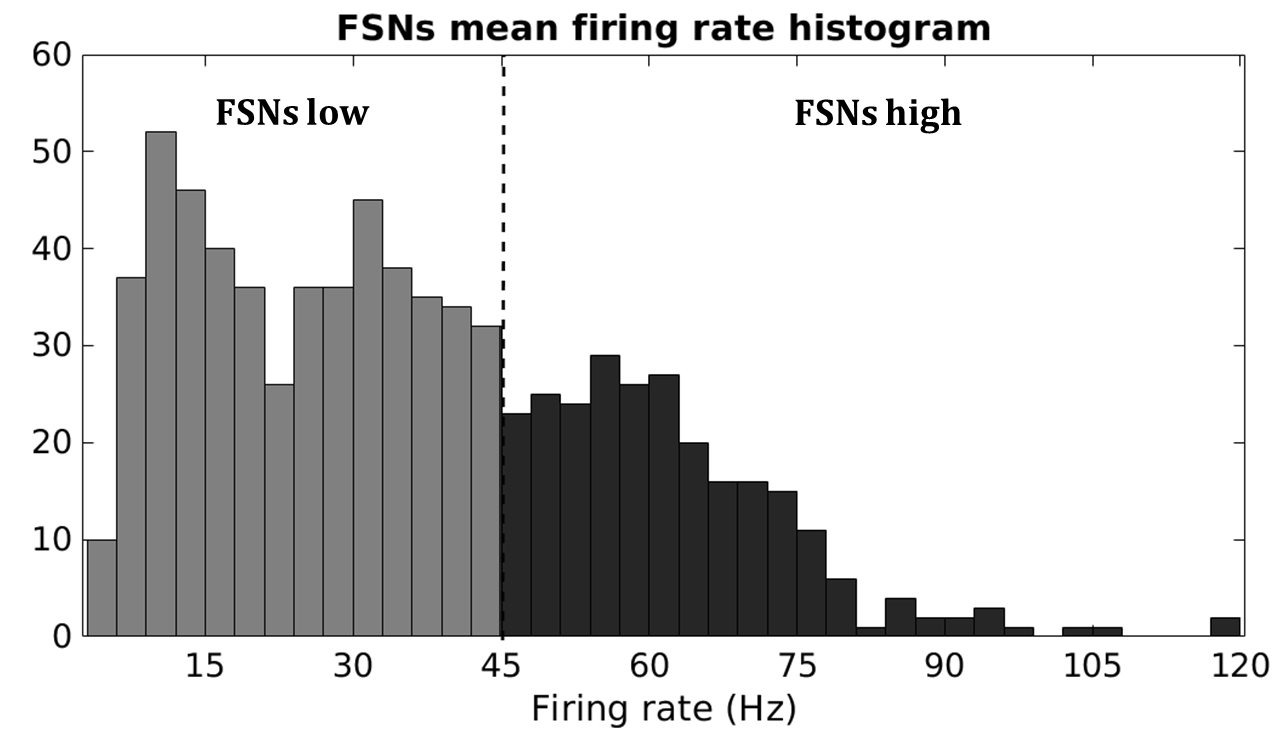
\includegraphics[scale=0.65]{figures/FSNFiringRateLightDark.pdf}
    \caption{Histogram of FSNs mean firing rate. I can distinguish two populations of FSNs: FSN$^{low}$ population, that are light grey in the graph, characterized by having firing rates below 45 Hz, FSN$^{high}$, in dark grey, characterized by having firing rates from 45 Hz upwards.}
    \label{fig:FSNsFireHisto}
\end{figure}
\begin{figure}
    \centering
    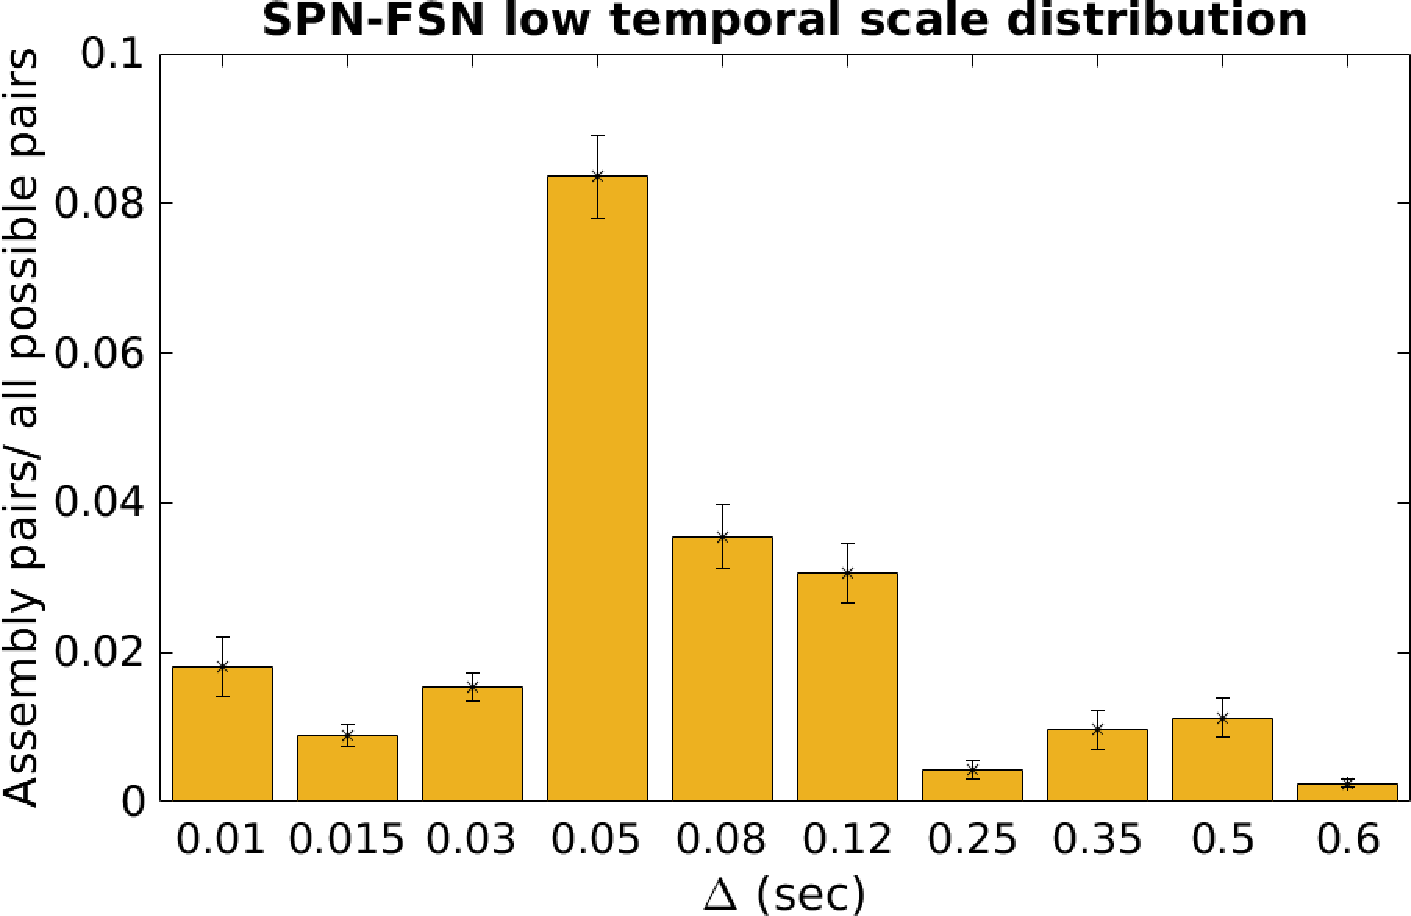
\includegraphics[scale=0.54]{figures/SPN_FSNlow1.pdf}
    \caption{SPN-FSN$^{low}$ temporal scale distribution peaked at 50 $ms$. With other frequent SPN-FSN$^{low}$ pairs detected also at 80 $ms$ and 120 $ms$.}
    \label{fig:SPN_FSNlowBin}
\end{figure}
\begin{figure}
    \centering
    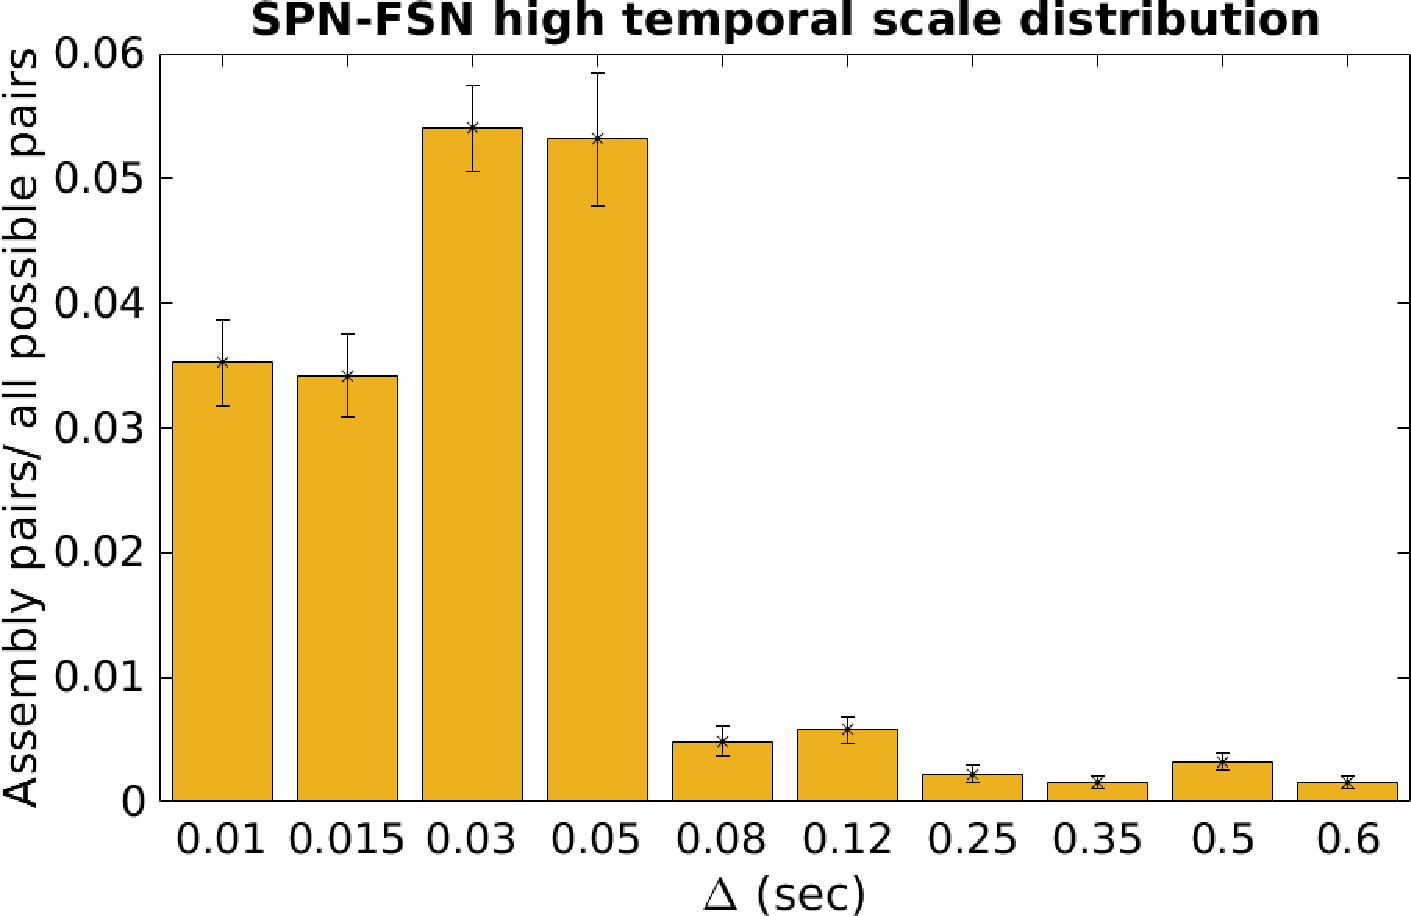
\includegraphics[scale=0.54]{figures/SPN_FSNhigh1.pdf}
    \caption{SPN-FSN$^{high}$ pairs were almost exclusively detected at very precise time scales, namely from 10 $ms$ to 50 $ms$.}
    \label{fig:SPN_FSNhighBin}
\end{figure}
In VS I noticed differences between SPN-FSN$^{low}$ pairs and SPN-FSN$^{high}$ bin size distributions. SPN-FSN$^{low}$ bin distribution peaked at 50-80 $ms$(figure \ref{fig:SPN_FSNlowBin}); whereas SPN-FSN$^{high}$ pairs were by-and-large only detected at more precise temporal scale (figure \ref{fig:SPN_FSNhighBin}).\\ I conclude that those two pair-types give specific contributions to the global VS-VS temporal scale distribution. The variety of time scales involved in intra- or cross- area interactions in the studied regions emphasizes the complexity of the interactions within the circuit.
\section{Directionality} 
\label{sec:Directionality}
 I had found in \hyperref[sec:TimeScales]{Section~\ref*{sec:TimeScales}} that interregional interactions have two characteristic time scales, which led us to consider more precise ($\Delta \in [0.01,0.25] ms$) and broader ($\Delta \in [0.25,0.6] ms$) time scales separately when examining the directionality of VS-VTA assembly-pairs.\\One of the output of the cell-assembly algorithm (CAD) is the inter-units activation lag of the assembly. When I restrict the investigation to interregional pairs, the lag modulus tells us the delay in activation between the two region while the sign of the lag indicates the direction of the activation, namely which region became activated first and which one follows.\\In figure \ref{fig:LagInSecAll} I show the lag distribution for the detected interregional assembly-pairs in the two characteristic time scales of interaction. As indicated in the plot, a positive lag means that VS is functionally leading the VTA activation and a negative lag indicates the opposite direction.\\The two lag distributions showed remarkable differences: the lag distribution of broader pairs was fat-long tailed, indeed, a substantial fraction of assembly-pairs detected had long activation lag ($lag > 1 sec$); more precise lag distribution had instead thin tails: almost all pairs detected in precise time scale had short lag ($|lag| < 1 sec$), and a good portion of pairs was detected within a lag value of 0.5 $sec$.\\I focused the study on the more precise temporal scales, first because in this way the temporal scale interactions were separated to typical task-related time scales, as e.g. the length of the odor duration, which covered typically an interval from 1.0 $sec$ to 1.5 $sec$. Secondly, the prediction error functions are expressed by dopamine circuit in short time scales (within 1 $sec$ from stimulus onset).\\ I used the cell-types classification presented in \hyperref[chap:UnitsAnalysis]{~Section \ref*{chap:UnitsAnalysis}} to divide the interregional assembly-pairs, according to their underlying cell-types (see \hyperref[sec:AsseTypes]{~Section \ref*{sec:AsseTypes}}). Doing so, I could divide the global lag distribution in lag distributions specific of those assembly-pair types. Figure \ref{fig:LagInSec4typo} shows the lag distribution for the four principal assembly-pair types.\\I observed a strong directionality in the assemblies composed of striatal projection neurons leading dopamine neurons (SPN-DAN pairs). All the other pair-types did not show a clear preferred directionality. Furthermore, inter-unit activation lags of assemblies containing pallidal neurons (FSN) and DAN were shorter (mean lag of 0.19 sec)than those containing SPN and DAN (mean lag of 0.26 sec), compatibly with assumed connectivity.\\VTA dopamine neurons were optogenetically tagged in first place, so I could use the tagged units as control to validate the dopamine neurons classification. Figure \ref{fig:LagInSecLaser} shows the lag distribution of laser tagged dopamine units coupled with SPN and FSN. Similar lag distributions were observed for pairs containing laser tagged DAN and pairs containing all DAN based on response classification. Indeed, SPN-DAN$^{laser}$ pairs showed directionality in direction $VS\rightarrow VTA$, whereas FSN-DAN$^{laser}$ were not directional, as I expected from the results obtained using units selected by the classification criteria, which confirms the validity of the adopted classification.\\
\begin{figure}[H]
\centering
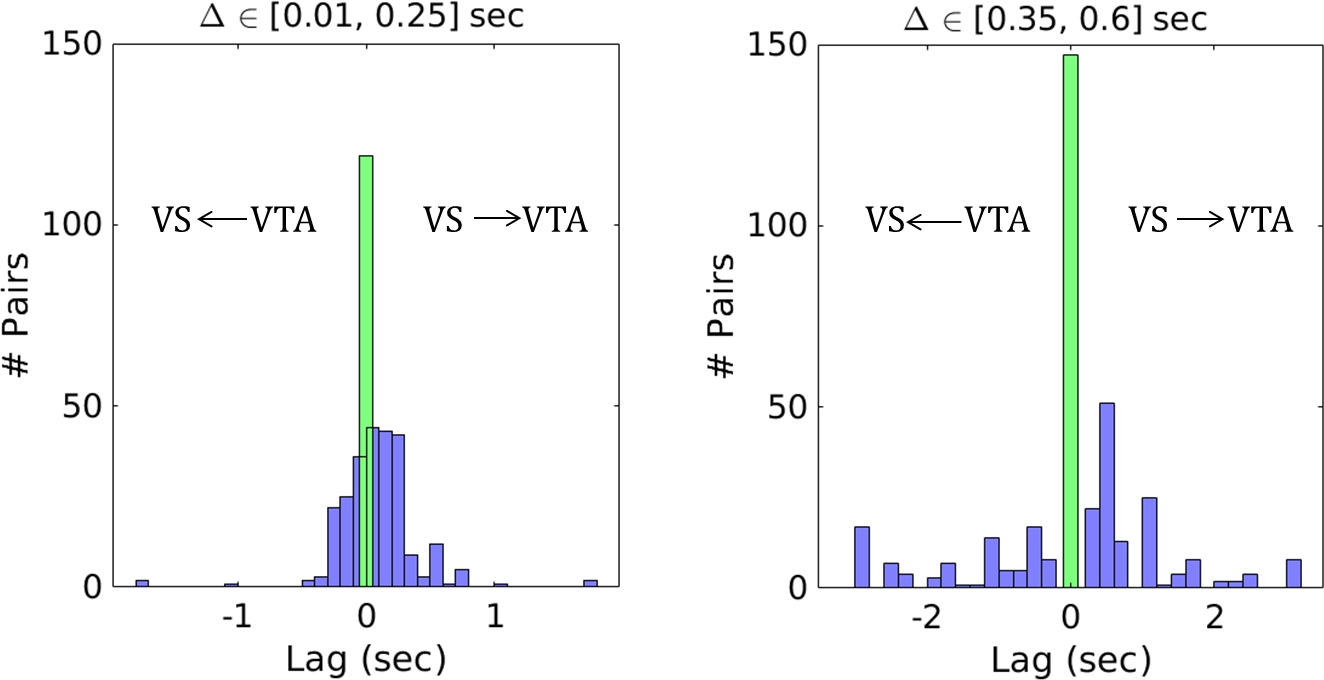
\includegraphics[scale=0.65]{figures/LagGeneral1.pdf}
\caption{Lag distribution for VS-VTA pairs in seconds. In green, the synchronous pairs. In violet, directional pairs. On the left, lag distribution of pairs detected in more precise time scale. On the right, the lag distribution for pairs detected in the broader time scale, presented with a fat-tailed distribution.}
\label{fig:LagInSecAll}
\end{figure}
\begin{figure}[H]
\centering
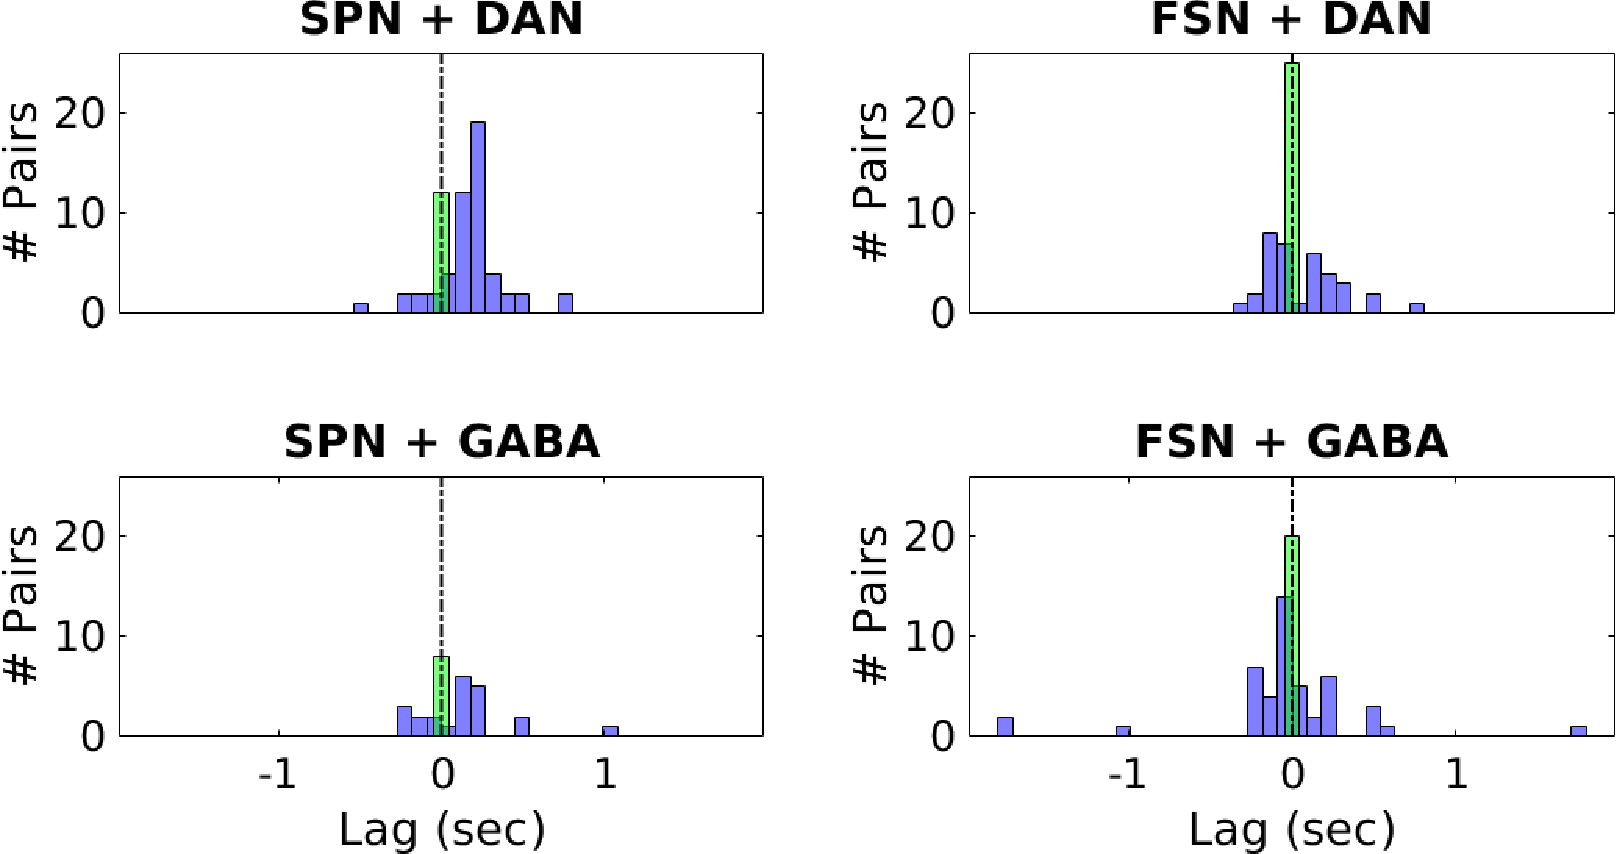
\includegraphics[scale=0.52]{figures/LagSec4Typo3VS.pdf}
\caption{Lag distribution of the four more represented pair-types in assemblies with precise time scales. Only SPN-DAN pairs show a preferred directionality, namely $VS\rightarrow VTA$.}
\label{fig:LagInSec4typo}
\end{figure}
\begin{figure}[H]
\centering
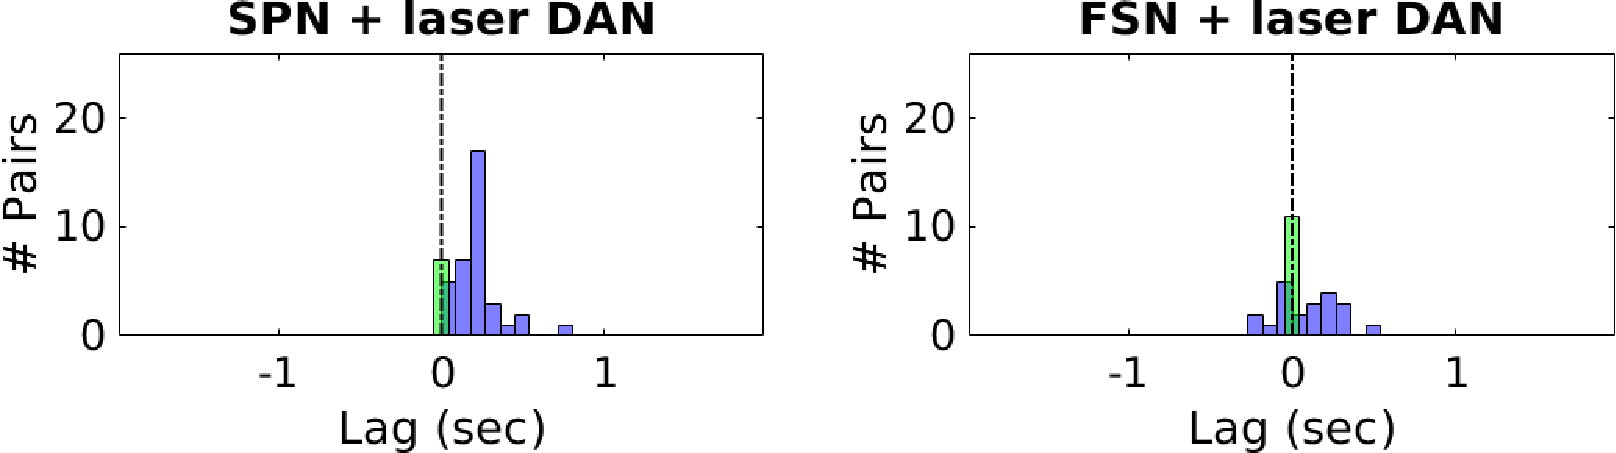
\includegraphics[scale=0.44]{figures/LagSecLaser3VS.pdf}
%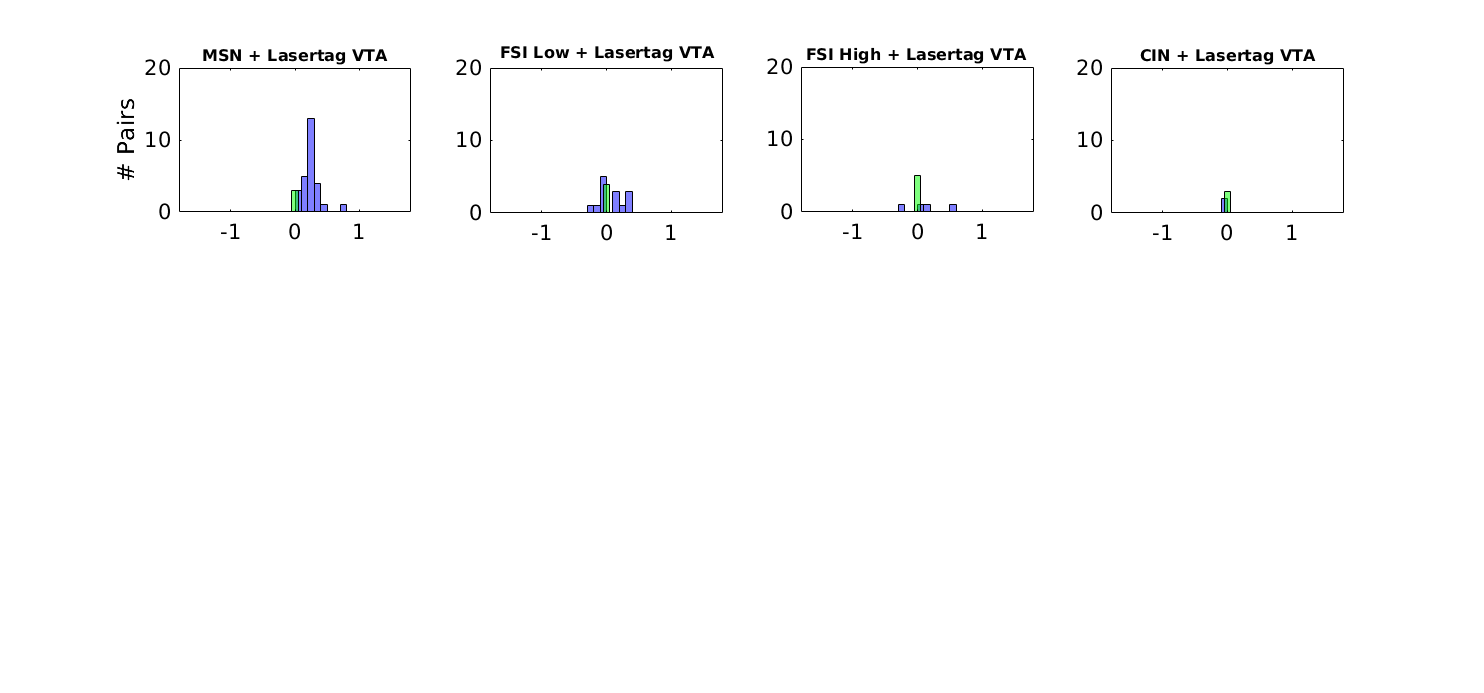
\includegraphics[scale=0.4]{figures/OnlyLaserOriz.pdf}
\caption{Lag distribution of DAN$^{laser}$ in pair with SPN and FSN units, in precise time scales. Lag distributions were similar to the lag distributions of classified DAN in pairs with SPN and FSN, confirming the directionality expressed by SPN-DAN pairs and the validity of the classification adopted in VTA.}
\label{fig:LagInSecLaser}
\end{figure}
The kind of activation exhibited by directional pairs is exemplified in figure \ref{fig:directional_assembly}. The pair in the example was detected with a bin width of $\Delta = 0.12 sec$, and the inter-units activation lag was positive $lag = 0.36 sec$. From the activation profile one can see that the illustrated assembly-pair specifically coded for the rewarded odor.\\Finally, looking at the activity of the two composing neurons, the directionality exemplified by the pair was evident: first the VS unit became actived and, after a temporal delay, the activation of VTA unit followed. Raster plots show how the activity across trials changed. In both units it is visible a gradient of activation across trials. In the first trials (less than 10 trials) the activity was either rare (VS unit), or uniform distributed in the odor window (VTA unit); after few trials, VS unit first, and later the VTA unit, showed a peak in activation at odor onset, that, then remained stable (figure \ref{fig:directional_assembly}).
\begin{figure}[H]
    \centering
    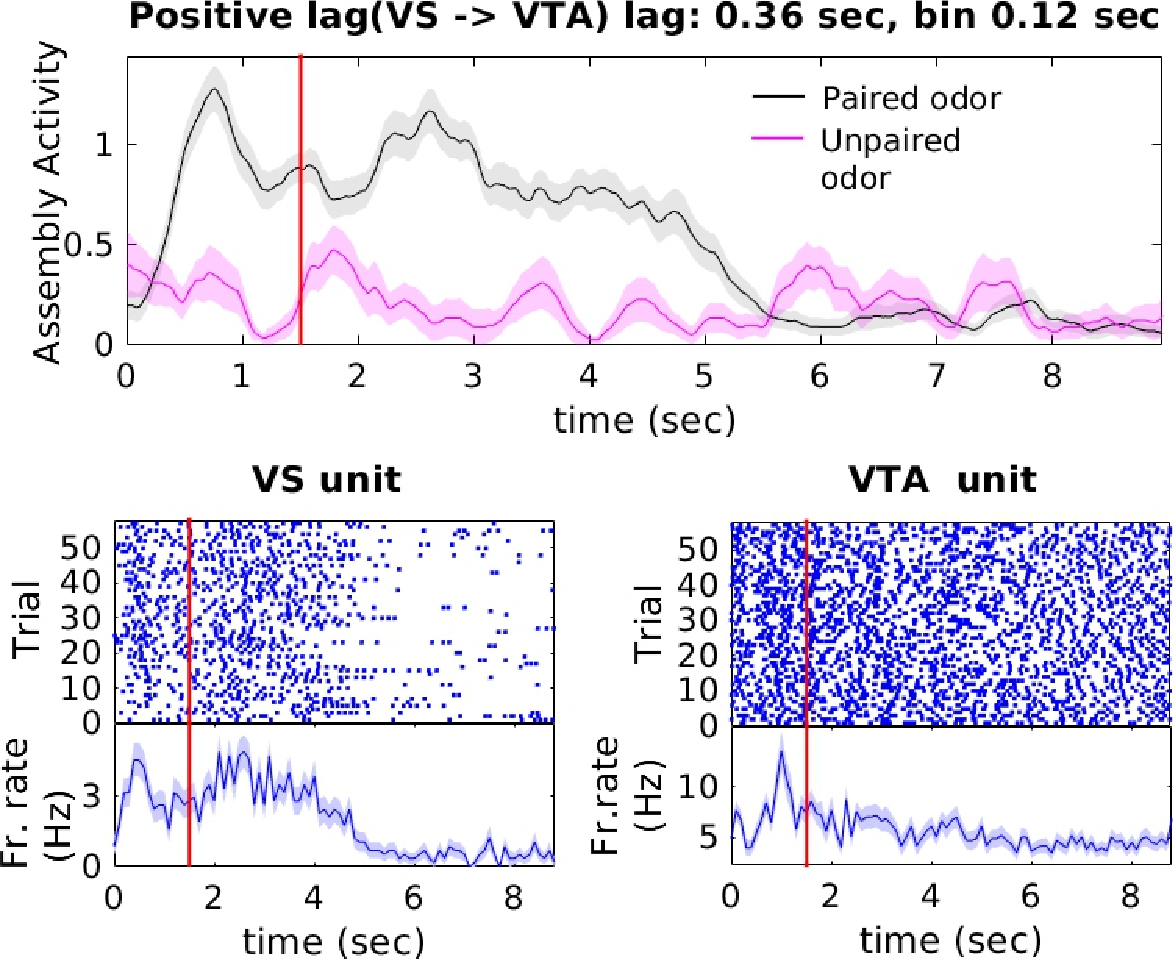
\includegraphics[scale=0.6]{figures/DirectionalAsEx1.pdf}
    \caption{Directional assembly.\textbf{Top:} mean across trails and standard error of the activity of the pair for the rewarded (grey) and unrewarded odor (purple) in the original phase. \textbf{Bottom:} raster plot and firing rate (mean and standard deviation) of units in an exemplary assembly-pair. x-axis origin corresponds to the odor onset, while the red line marks the end of the stimulus duration. The examined assembly had a positive lag, that means VS preceding in activity VTA. In the neuronal firing activity the VS unit activated before than the VTA unit.}
    \label{fig:directional_assembly}
\end{figure}
At the population level, time scale and directionality segregation revealed multiple assembly-activation patterns. In figure \ref{fig:AsActBinLag} it is shown an example of activation patterns for the interregional assembly-pairs activity averaged across trials\footnote{The activation $\mathcal{I}$ ranges in the interval $[0,1]$, after normalized as follows:
\begin{equation}
    \mathcal{I} = \frac{I-\min(I)}{\max(I)-\min(I)}
    \label{eq:norm}
\end{equation} were $I$ is the not normalized activity.}. 
Assembly-pairs exhibiting directionality $VS \rightarrow VTA$ and detected in the precise time scale ($\Delta \le 0.25$) became activated early during the odor presentation.\\The early activation at the stimulus presentation is the type of activation expected when animals predict the reward. As discussed in \hyperref[chap:Introduction]{Chapter ~\ref*{chap:Introduction}} (see also figure \ref{fig:probDopamine}), reward-related responses in DAN changed as the reward probability change. The typical prediction error signal is presented as an high activation at the stimulus presentation in case of high reward probability, and less activation at the retrieval. Moreover I have shown in figure \ref{fig:LagInSec4typo} that the SPN-DAN assembly-pairs were directional, thus I speculated that SPN-DAN were good candidate for reward prediction error coding; the investigation of this hypothesis will be argument of the next chapters.
\begin{figure}[H]
    \centering
    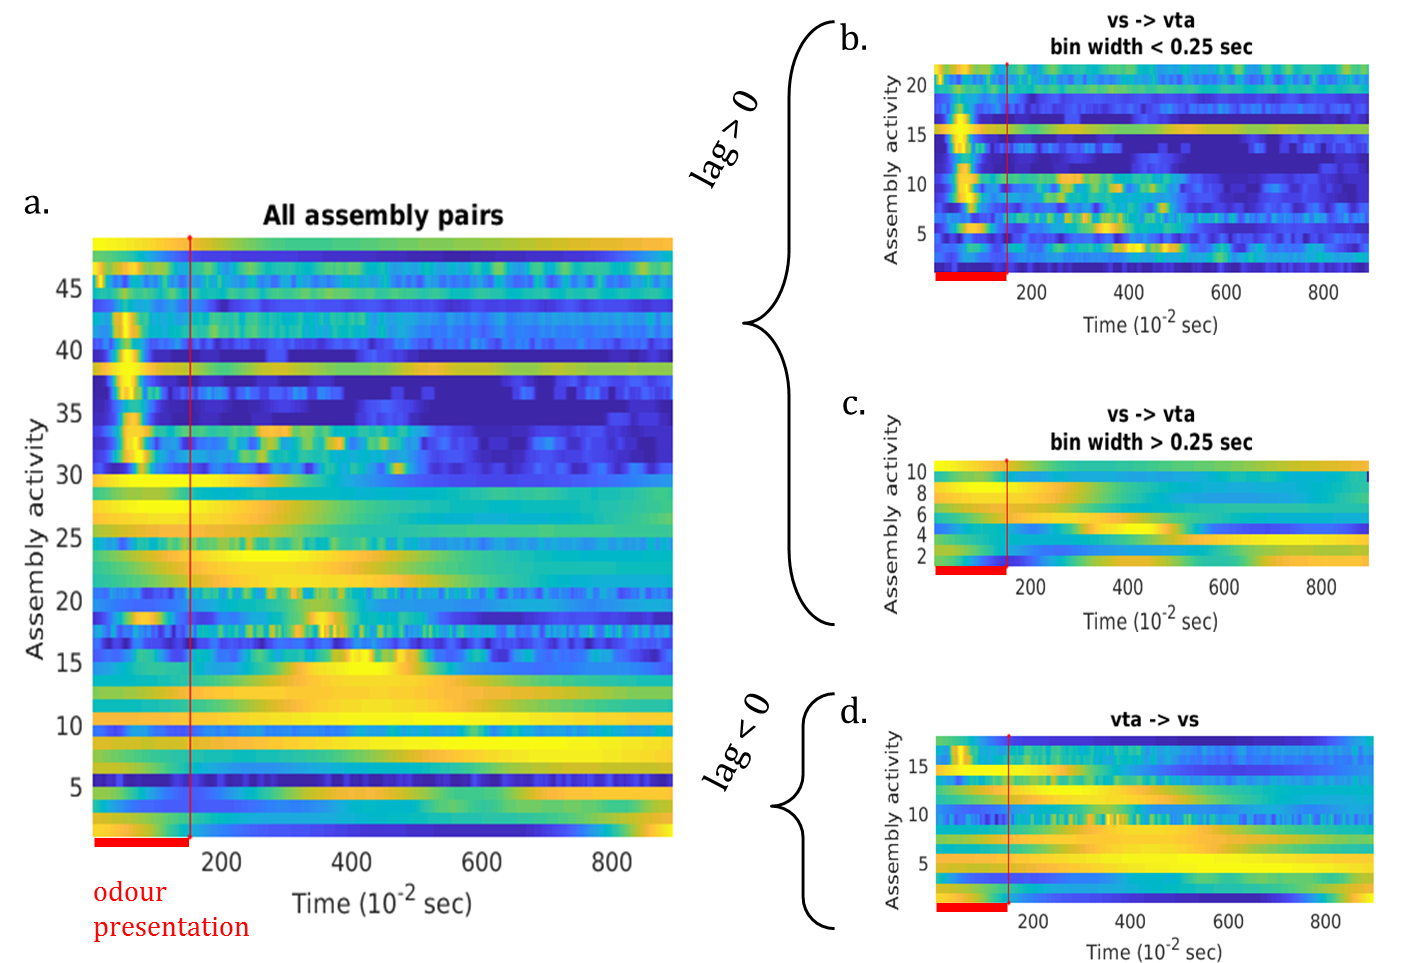
\includegraphics[scale=0.56]{figures/AsActPerBinLag1.png}
    \caption{Assembly-activation patterns given time bins and lags. In (a.) heat map of the activation of interregional pairs in one the experimental paradigms. The activation is normalized in such a way the activity range is $[0,1]$. Color scale ranges from deep blue, indicating the minimum possible, to yellow, indicating high activity. Pairs from (a.) were selected for bin size ($\Delta$) and lag: $\Delta < 0.25 s$ and $lag > 0$ (b.), $\Delta > 0.25 s$ and $lag > 0$ (c.), $lag < 0$ (d.)}
    \label{fig:AsActBinLag}
\end{figure}
\section{Conclusion}
From the time scale distribution of interregional assembly-pairs emerged that VS-VTA assembly-pairs consisted in two classes of interactions, highlighting the complexity of the VS-VTA pair interactions and the importance of accounting for temporal precision when studing neuronal assemblies.\\The two time scales involved in VS-VTA interaction were separated to study the lag analysis, revealing a preferred directionality $VS\rightarrow VTA$, specifically in pairs containing striatal projection neurons and dopamine neurons.\\Different time scales of interaction and directionalities reflect different patterns of assembly-pair activity. Pairs detected at the precise time scale exhibited the directionality $VS\rightarrow VTA$ with a prominent activation during the stimulus presentation, as expected for prediction error signals.\\Since directional assemblies are formed by striatal projection neurons and dopamine neurons, I hypothesized that those pairs are good candidates for prediction coding. The next chapter is aimed to understand whether SPN-DAN assembly-pairs compute specifically prediction error signals. Comparing the activity of different assembly-pair types I therefore ask whether different assembly-pair types specialize in different coding features.
 \section{Pair-types task-related pattern}
 \label{sec:TaskResp}
In the previous section I concluded that the time scale segregation and the directionality of VS-VTA assemblies might reflect specific task-related coding feature. As an example I have shown how, for a specific dataset, different time scales and directionalities revealed different assembly-pair activity patterns. I have seen as well that different assembly-pair types have different directionality distribution. SPN-DAN assembly-pairs, in particular, exhibited a clear $VS\rightarrow VTA$ directionality, so I expect those assembly to have different patterns of activity with respect to other assembly-pair types.\\In this section I will test more sistematically whether different assembly-pairs-types have different task-related activity patterns, and consequently, express different coding functions.\\
To this purpose, I tested the responsiveness of each assembly-pair to the conditioned stimulus (CS $+/-$) and the unconditioned stimulus (US), through an analysis of variance performed on the assembly activity in four window of interest. I used both a paired Friedman test and a repeated measures ANOVA, corrected with tied-rank transformation to avoid parametric assumption. The results of the two tests were consistent each other (not shown). I choose to present here only Friedman test results, as it is free from gaussianity assumptions.\\Time intervals were 0.5 $sec$ long, and were chosen as follows: CS $+/-$ interval included all time steps $t \in [0, 0.5]$ $sec$ from the odor onset, CS$+/-_{cont}$. was the window including each time $t$ with $t \in [-0.5, 0]$ $sec$ before the reward retrieval, in which the the odor was still present, US interval included times $t \in [0,0.5]$ $sec$ from the reward delivery. The assembly-pair activity in the listed task relevant intervals was compared with the baseline activity ($t \in [-0.8, -0.3]$ $sec$ before the odor onset). Figure \ref{fig:Baseline} shows the heat map of the neural activity averaged across trials before and after the odor onset. During the baseline period (interval delimited by the two back lines) no activity patterns emerge besides the spontaneous neural activity.
\begin{figure}[H]
\centering
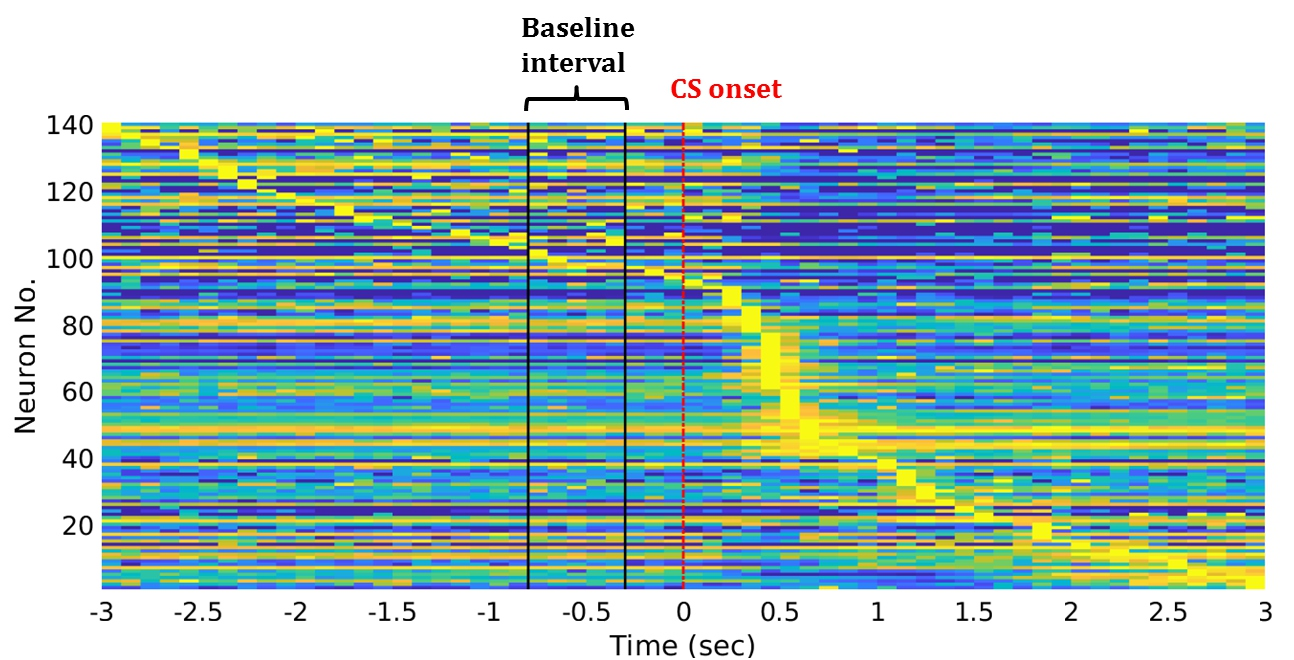
\includegraphics[scale=0.6]{figures/Baseline.pdf}
\caption{Baseline interval choice. Neural activity averaged across trials. For each trial the baseline interval was a time window in which no task related activity could have interfered with the spontaneous neural activity. Color map ranges from blue to yellow indicated with blue the minimum of activity and in yellow the maximum.}
\label{fig:Baseline}
\end{figure}
For each assembly-pair type I performed a large number of statistical tests, some will have p-values less than $0.05$ purely by chance, even if all null hypotheses of the family of tests performed are really true. Hence, Bonferroni correction for multiple comparison was applied (\cite{Bonferroni}, \cite{Dunn1958}, \cite{Dunn1961}). The Bonferroni correction is the classical approach to take in account the multiple comparison problem and consists in having a control on the familywise error rate ($\alpha=0.05$). This was achieved by setting the critical value $\alpha$ for an individual test at lower value than 0.05 in such a way that, if all the null hypotheses are true, the probability that the family of tests includes one or more false positives due to chance is 0.05. The value $\alpha$ for an individual test is obtained by dividing the familywise error rate by the number of tests.\\Analysis of variance compares the means of several groups to test the hypothesis that they are all equal, against the general alternative that they are not all equal. To compare the activity of specific  windows I hence performed a post-hoc test, Bonferroni corrected for multiple comparison.\\In figure \ref{fig:PercAsFried} the fraction in percentage of assemblies significant for Friedman test. The histograms refer to the Friedman tests made on hit trials, in original and reversal phase separately.
\begin{figure}[H]
\centering
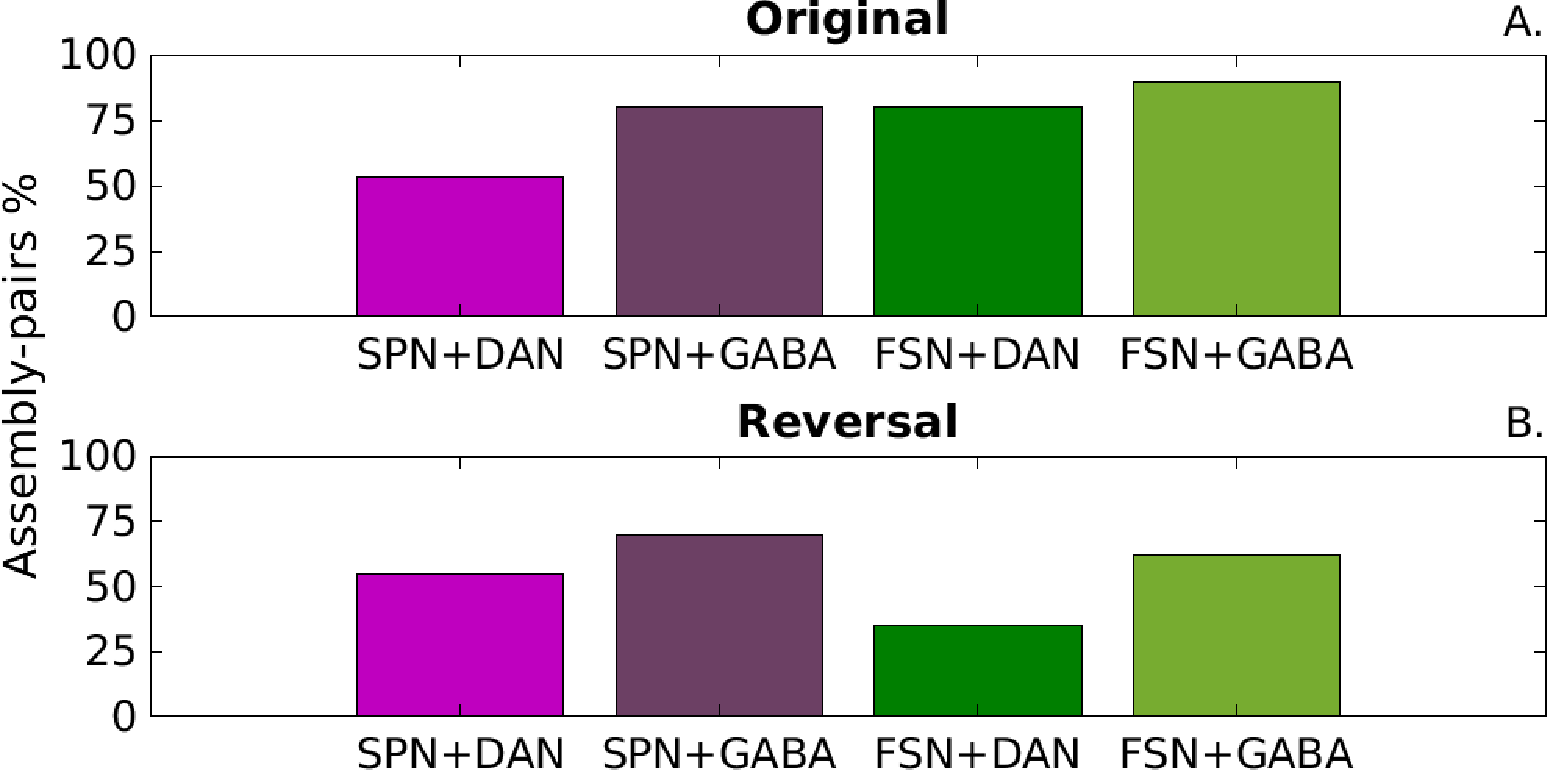
\includegraphics[scale=0.5]{figures/PercFriedHitTrialsBFf.pdf}
\caption{Percentage of assembly-pairs exhibiting a significant task related pattern activity. The Bonferroni correction for multiple comparison was applied. In A. the significant assembly-pairs tested for the original phase, in B. the significant assembly-pairs tested in reversal. Assembly are divided in the four principal pair-types.}
\label{fig:PercAsFried}
\end{figure}
\begin{figure}[H]
    \centering
    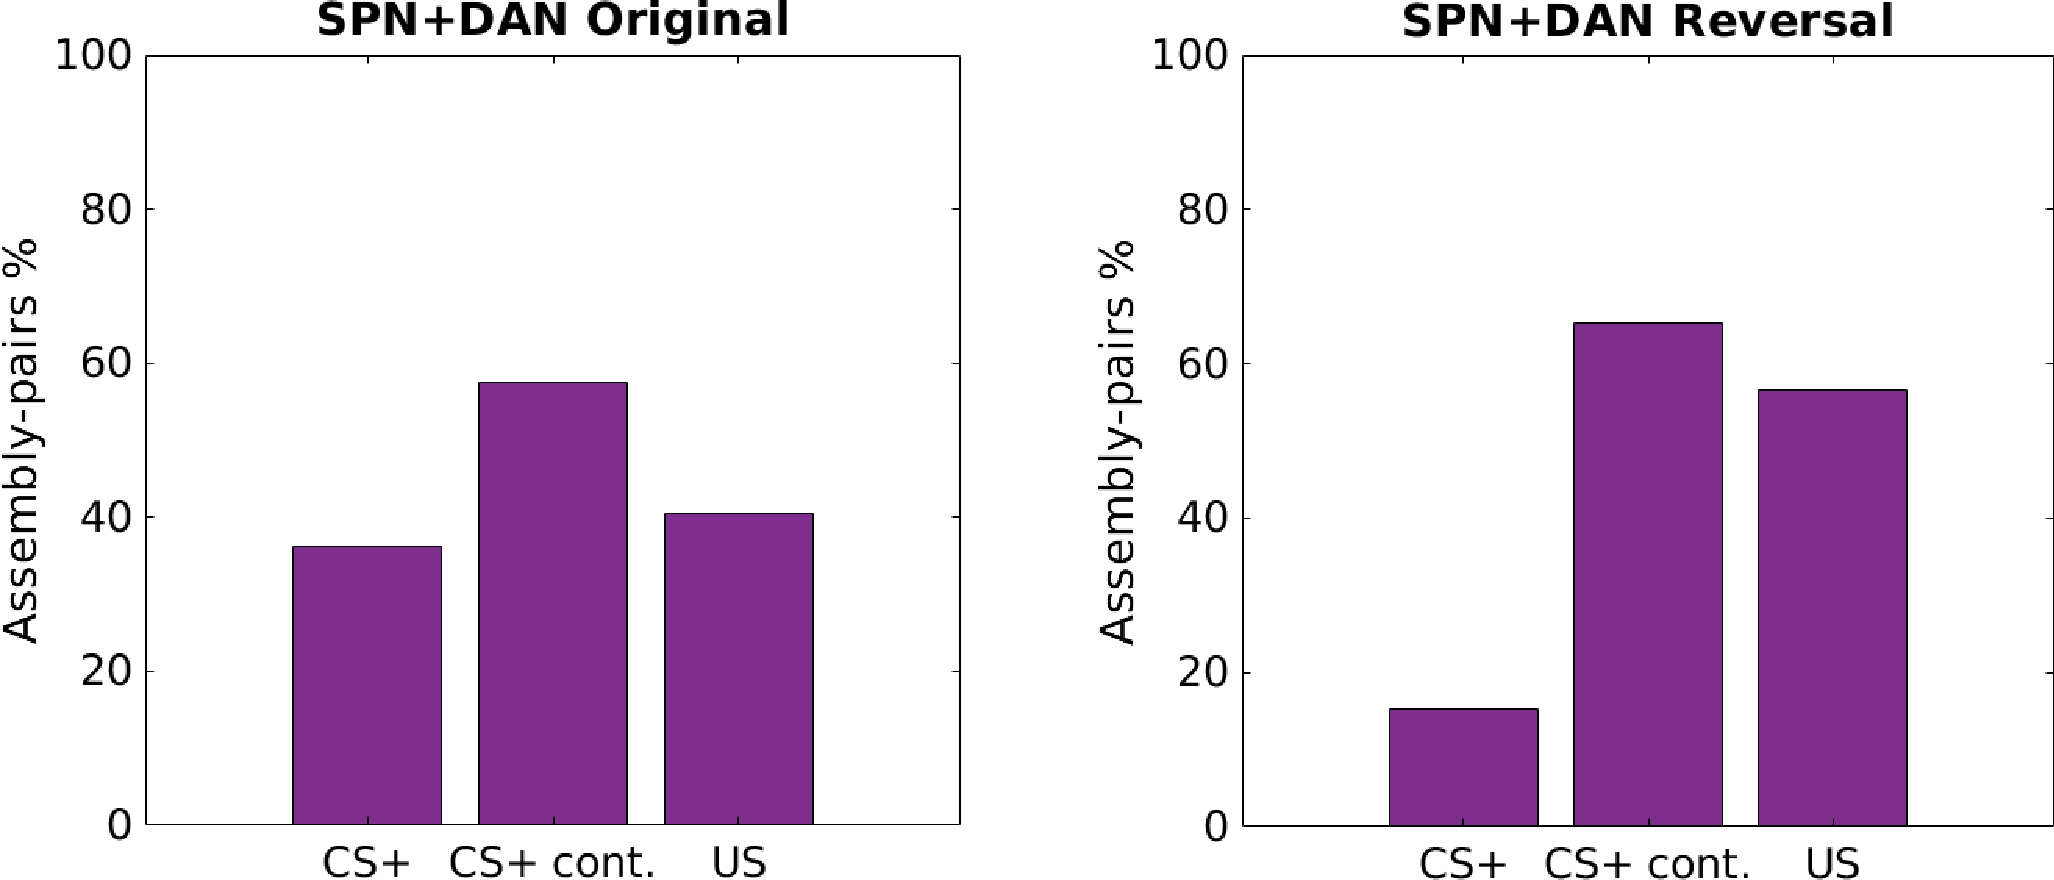
\includegraphics[scale=0.3]{figures/SPN_DANHisto.pdf}
    
    \vspace{1cm}
    
    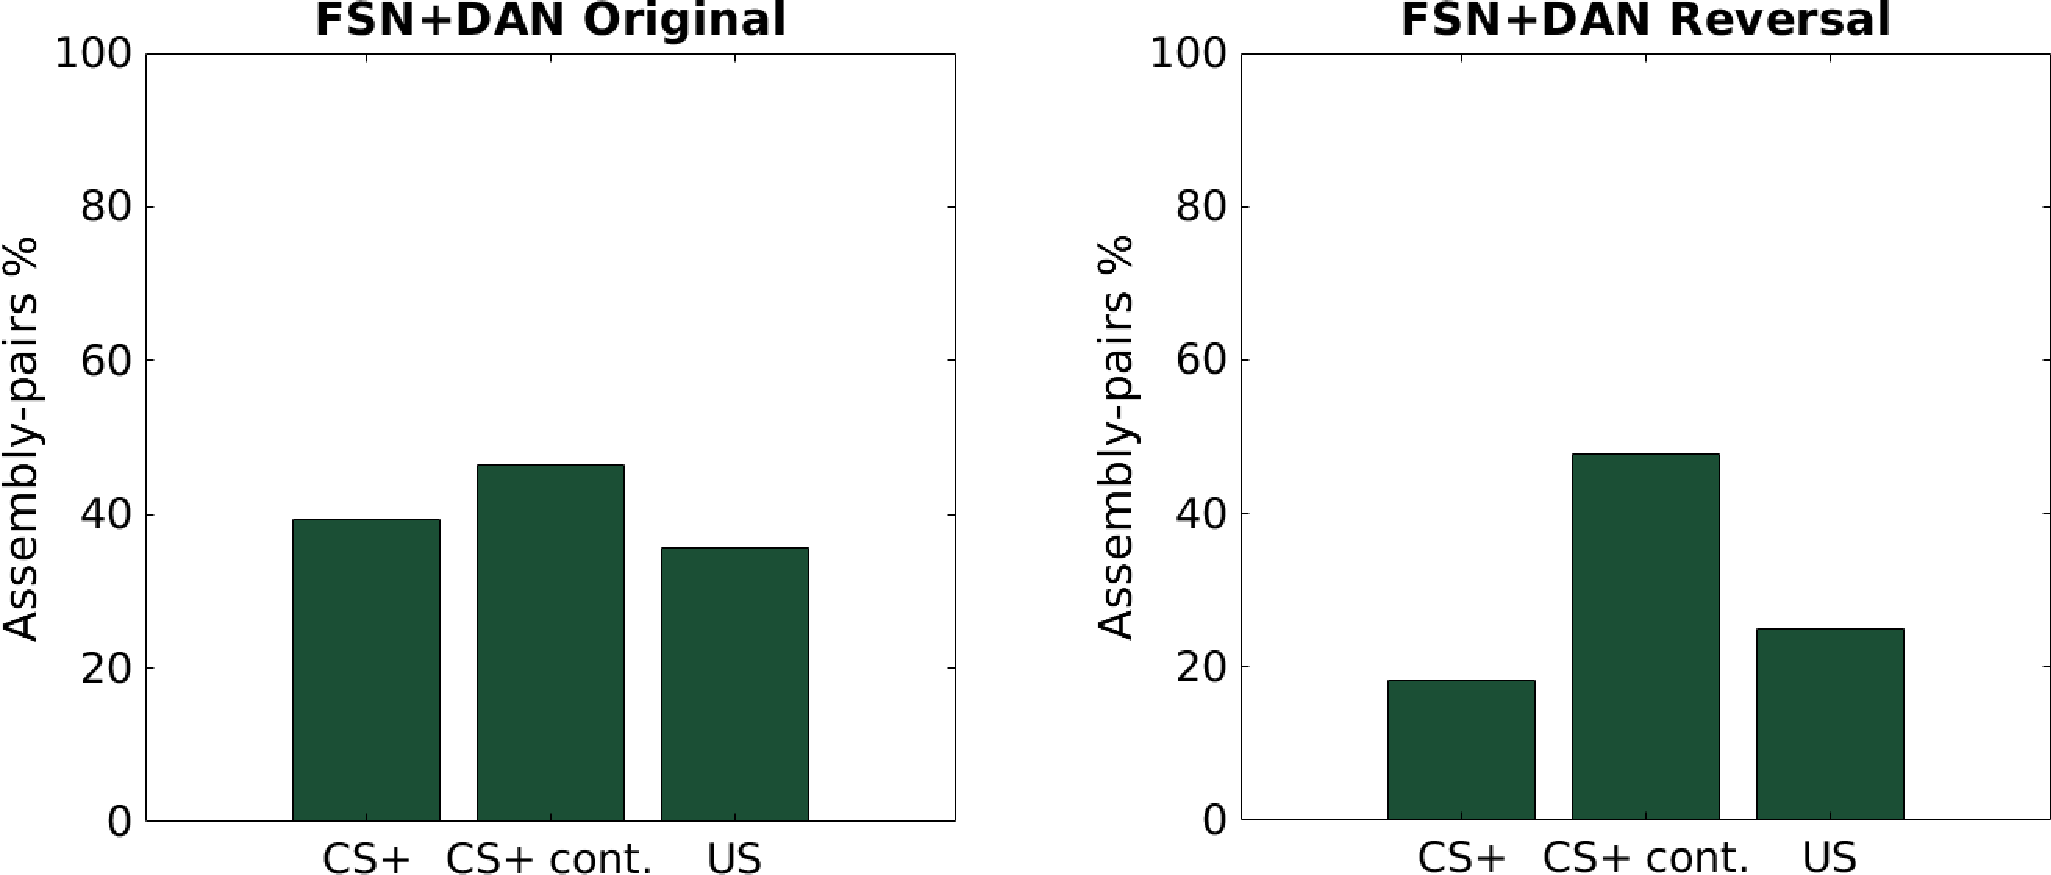
\includegraphics[scale=0.3]{figures/FSN_DANHisto.pdf}
    
    \vspace{1cm}
    
    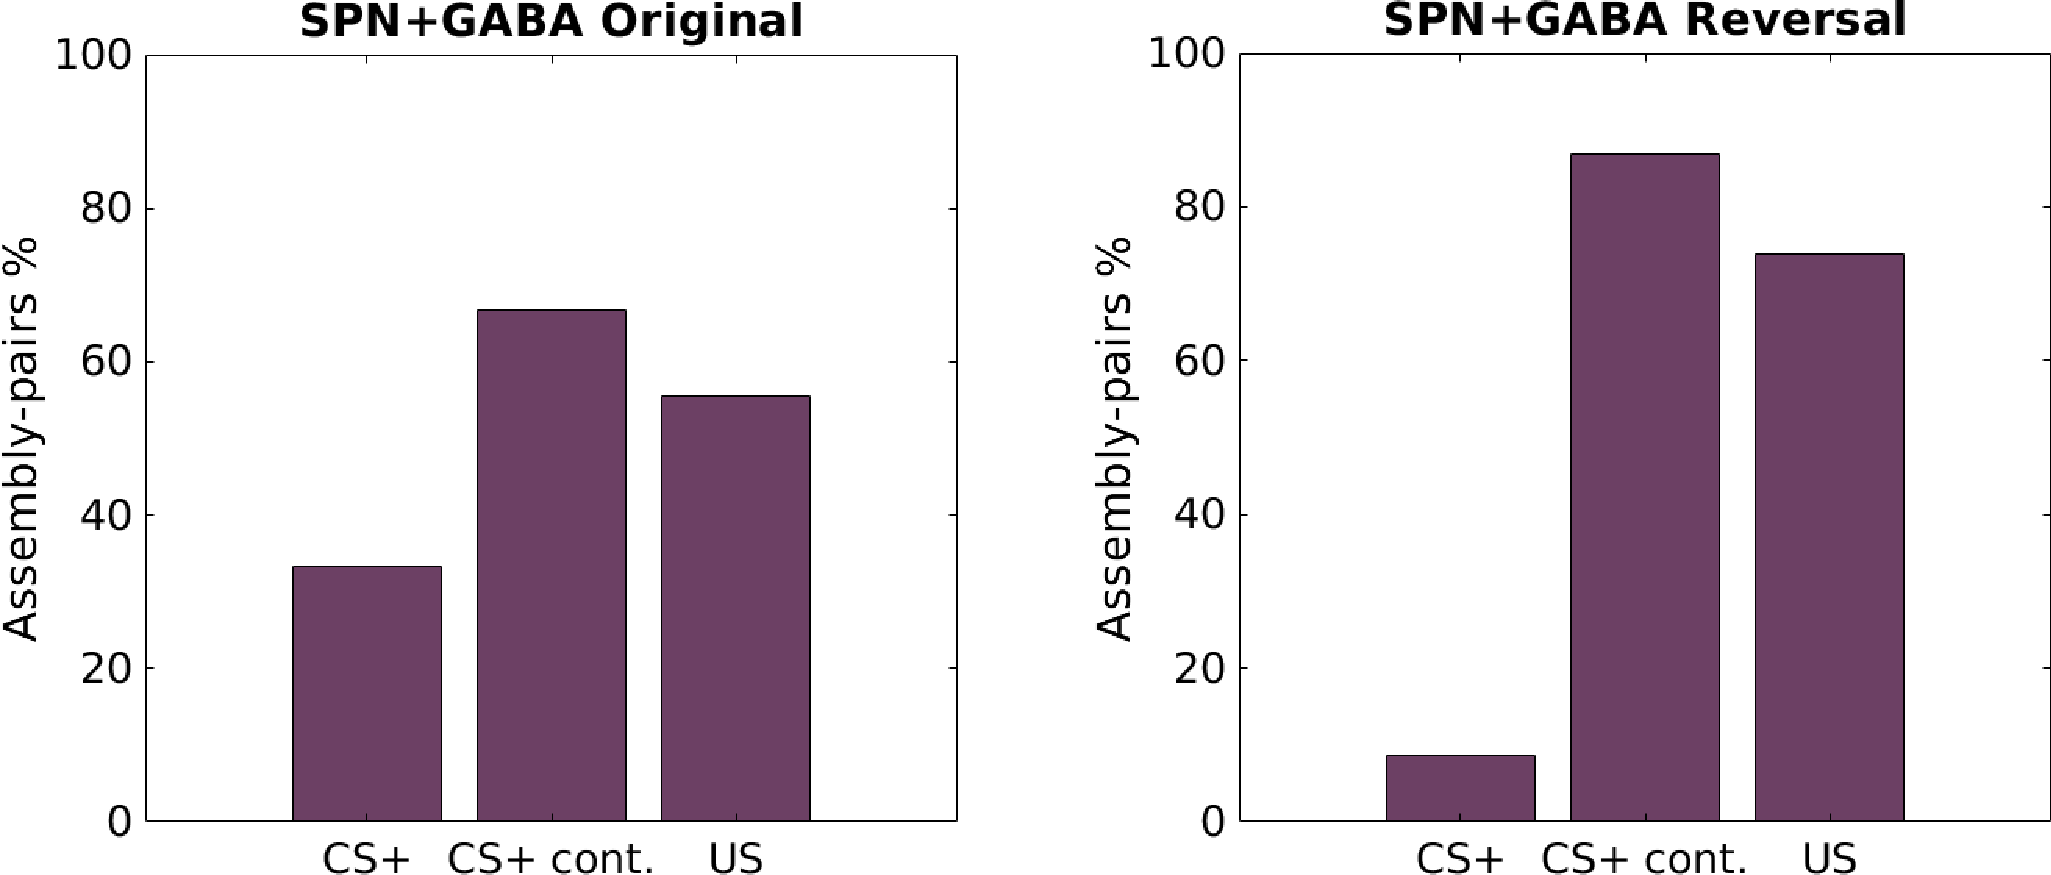
\includegraphics[scale=0.3]{figures/SPN_GABAHisto.pdf}
    
    \vspace{1cm}
    
    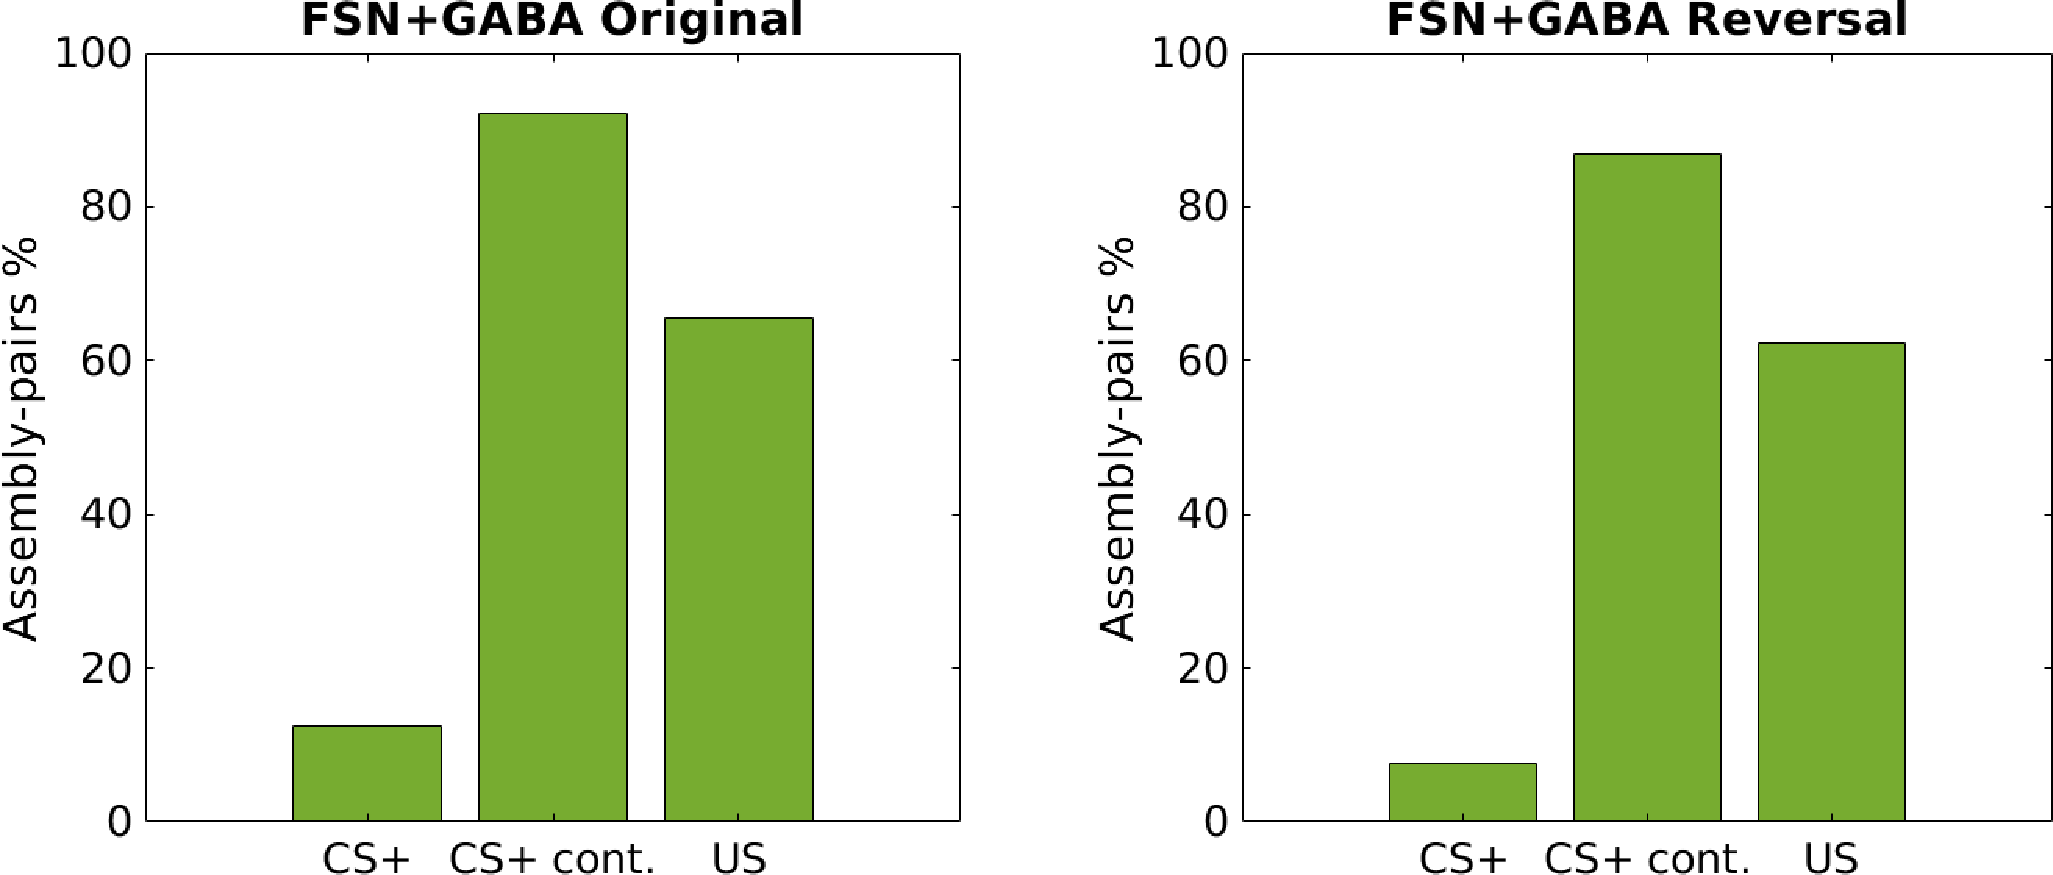
\includegraphics[scale=0.3]{figures/FSN_GABAHisto.pdf}
\caption{Percentage of assembly-pairs significant with respect to the baseline in the windows CS+, CS+$_{cont.}$, US. The total amount can exceed the $100\%$ since a same assembly could be found significant in multiple task window.}
    \label{fig:FriedHistoDAN}
\end{figure}
Different assembly-types were active in different task moments, summary plots are shown in figure \ref{fig:FriedHistoDAN} where I reported in which windows (CS+, CS+$_{cont.}$, US) assembly-pairs are significantly active with respect to the baseline. The total amount can exceed the $100\%$, since pairs could be found significant in multiple windows.\\All assembly-pair types were predominantly active in the window CS+$_{cont.}$, that is the window of preparation for the retrieval. There were differences among assembly-pair types and phases. The first remarkable difference is between the original and the reversal phase: in the reversal phase all pair-types were less activated in CS+ window with respect to the original phase.\\Differences in assembly-pair types emerged as well plotting the activity patterns of significant assemblies. Figure \ref{fig:HeatPairsDan} shows the activation profile of all assembly-pairs found significant in the original phase. In order: in figure \ref{fig:HeatPairsDan} (top-left) SPN-DAN assembly-pairs in original phase: a good portion of those pairs became active early at the rewarded stimulus (CS+) presentation, a good portion remained active during the stimulus presentation (CS+$_{cont.}$). Only a small fraction was active only in reward retrieval window (US). In figure \ref{fig:HeatPairsDan} (top-right) the same assembly-pairs in the reversal phase.\\FSN-DAN assembly-pairs on contrast have a phasic early response either to the rewarded stimulus (CS+) or reward retrieval (US) (figure \ref{fig:HeatPairsDan}, bottom-left); figure \ref{fig:HeatPairsDan} (bottom-right) shows the activation of the same FSN-DAN pairs in the reversal phase. With respect to the original phase I noticed less activation at CS+ and more at US.\\In assembly-pairs including SPN the decrease in activity in CS+ corresponded to more activity at retrieval (US) in the reversal phase, reflecting the reward-related surprise, expected to be more accentuated in reversal phase. Assembly-pairs composed of GABA units (figure \ref{fig:HeatPairsGaba}) became activated later than assembly-pairs containing DAN, and they were broadly active before the reward and during the reward consumption. Pairs with GABA or DAN were predicted to encode different signals, and indeed showed different task related patterns.
 \begin{figure}[H]
     \centering
     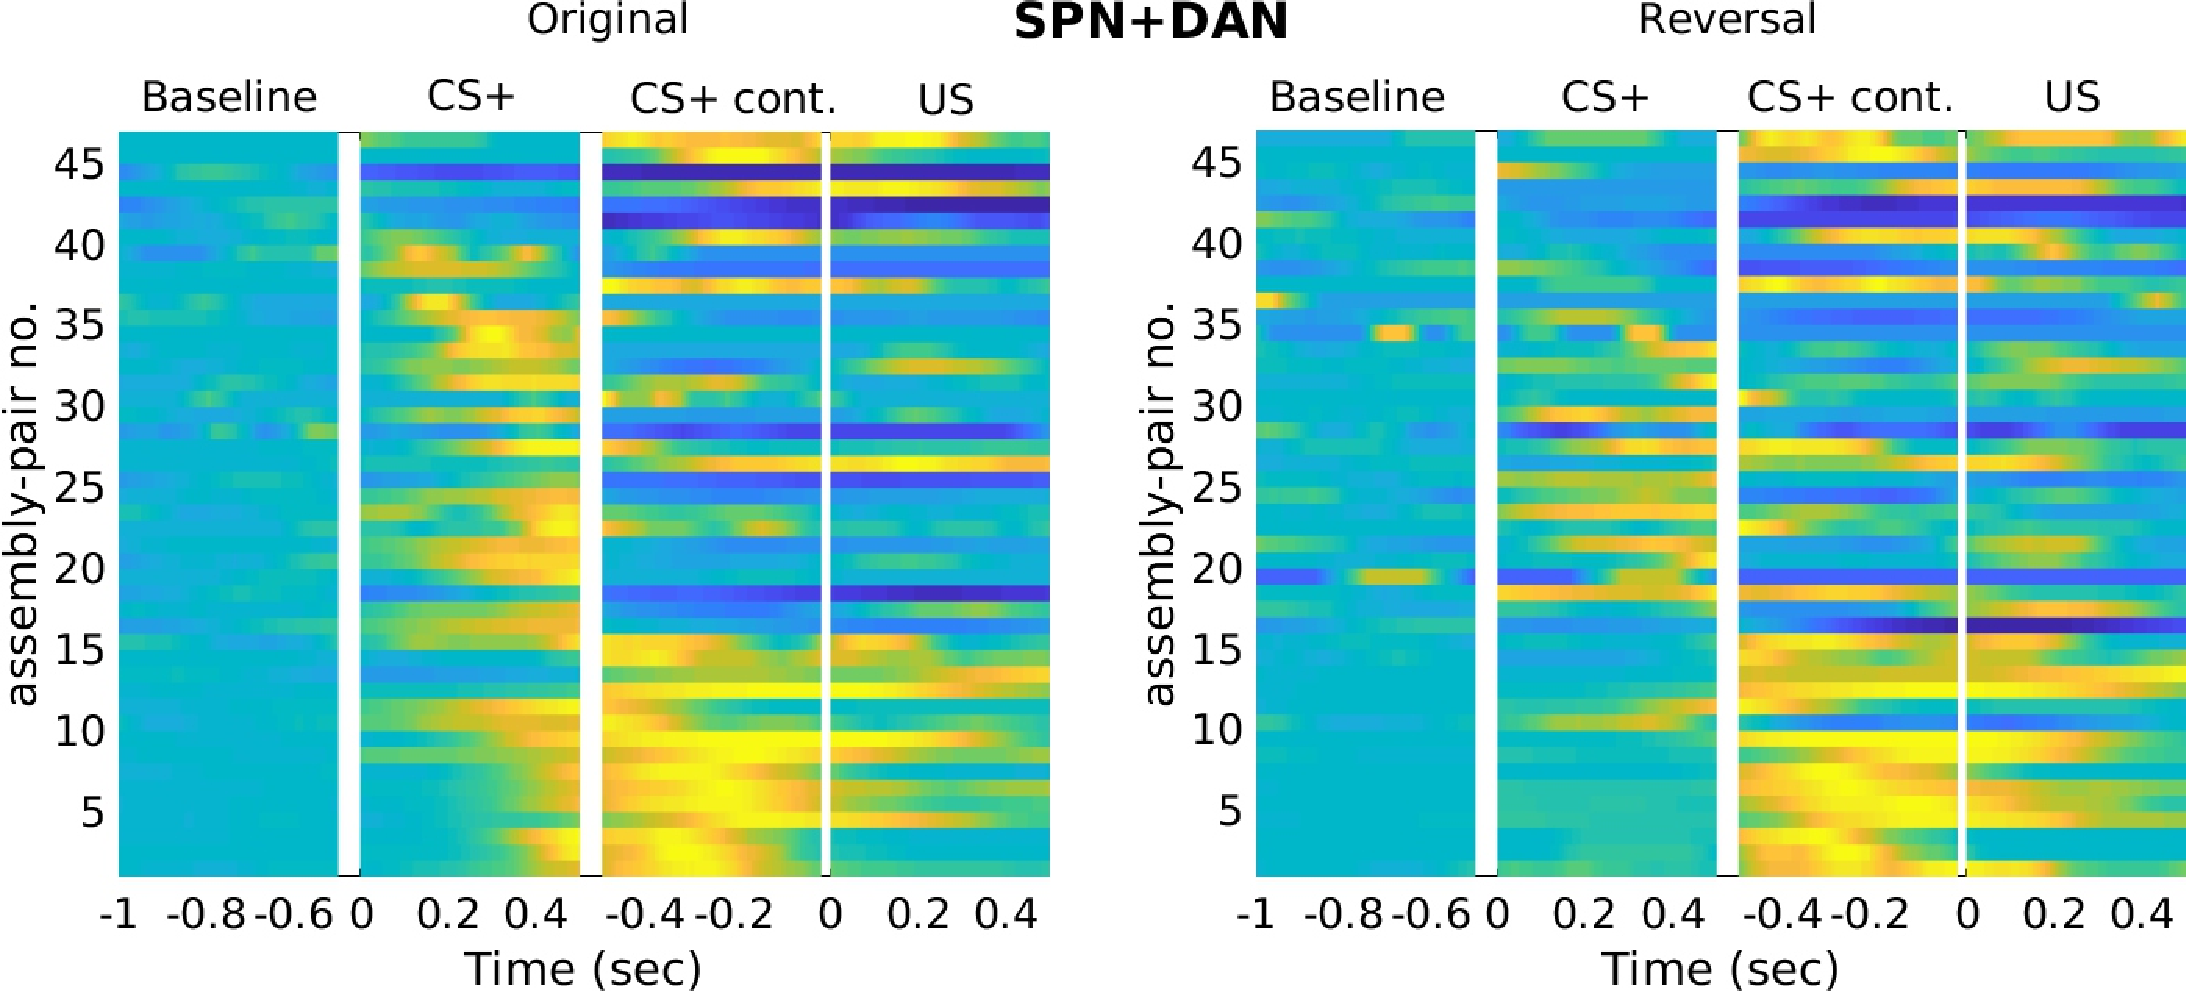
\includegraphics[scale=0.42]{figures/SPN_DAN.pdf}
     
     \vspace{1cm}
     
     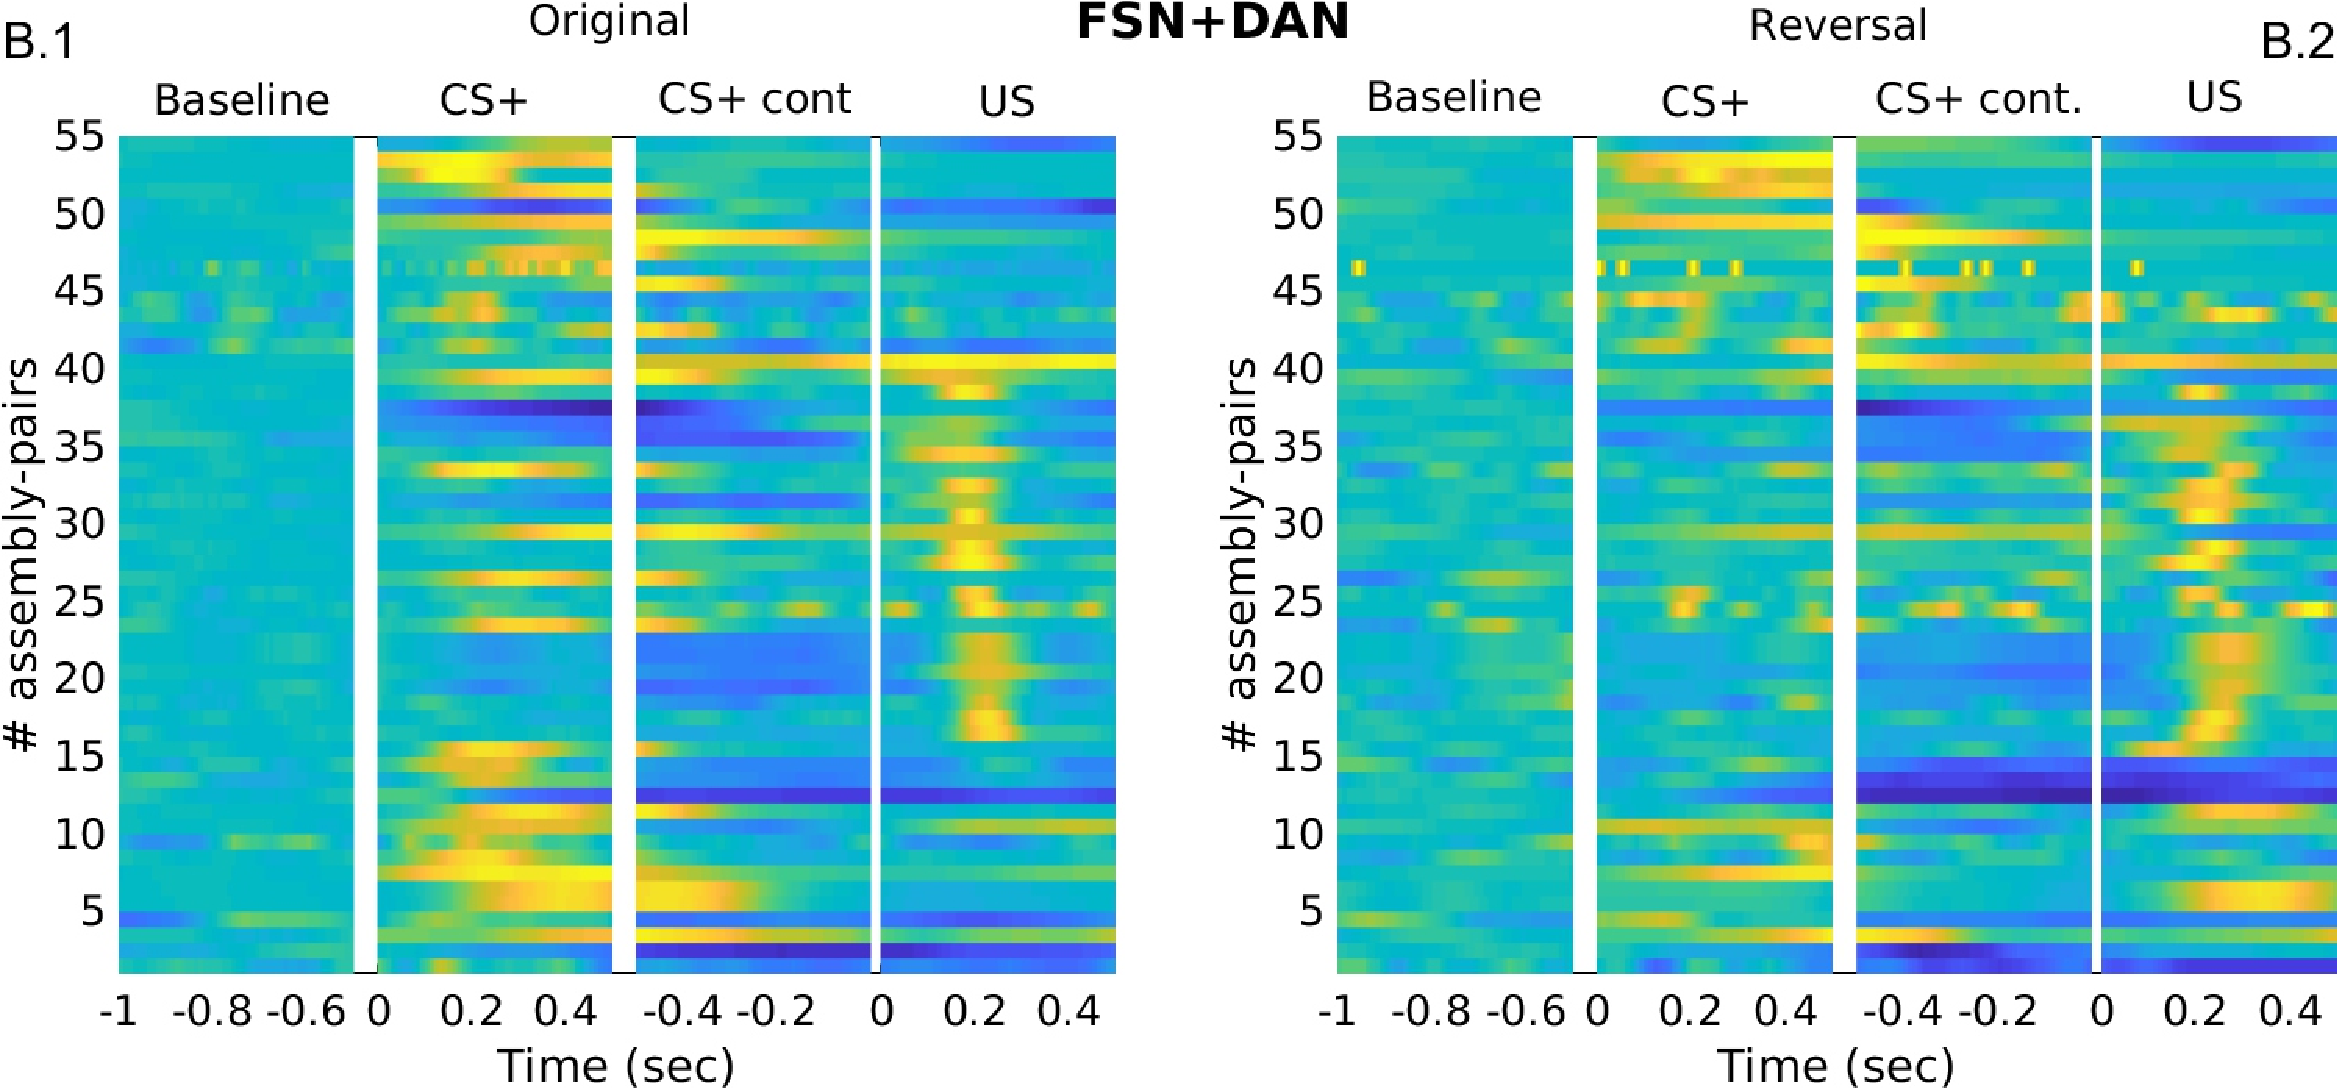
\includegraphics[scale=0.42]{figures/HeatFSN_DAN.pdf}
     \caption{Assembly-pairs tested with Friedman test with significant task related response in original phase. In order: \textbf{Top left:} SPN-DAN assembly-pairs; \textbf{top right:} the same assembly-pairs in the reversal phase. \textbf{Bottom left:} FSN-DAN assembly-pairs; \textbf{bottom right:} same FSN-DAN pairs in the reversal phase. The color map ranges from blue to yellow, indicating in deep blue inhibition, in turquoise almost no activation and in yellow high activation.The activity was normalized as in eq. \ref{eq:norm} were $\max(I)$ ($\min(I)$) was the absolute maximum (minimum) of assembly-activity among the four windows; the mean of the baseline was subtracted to each assembly. The maximum (minimum) is marked in yellow (deep blue).}
     \label{fig:HeatPairsDan}
 \end{figure}
 \begin{figure}
     \centering
     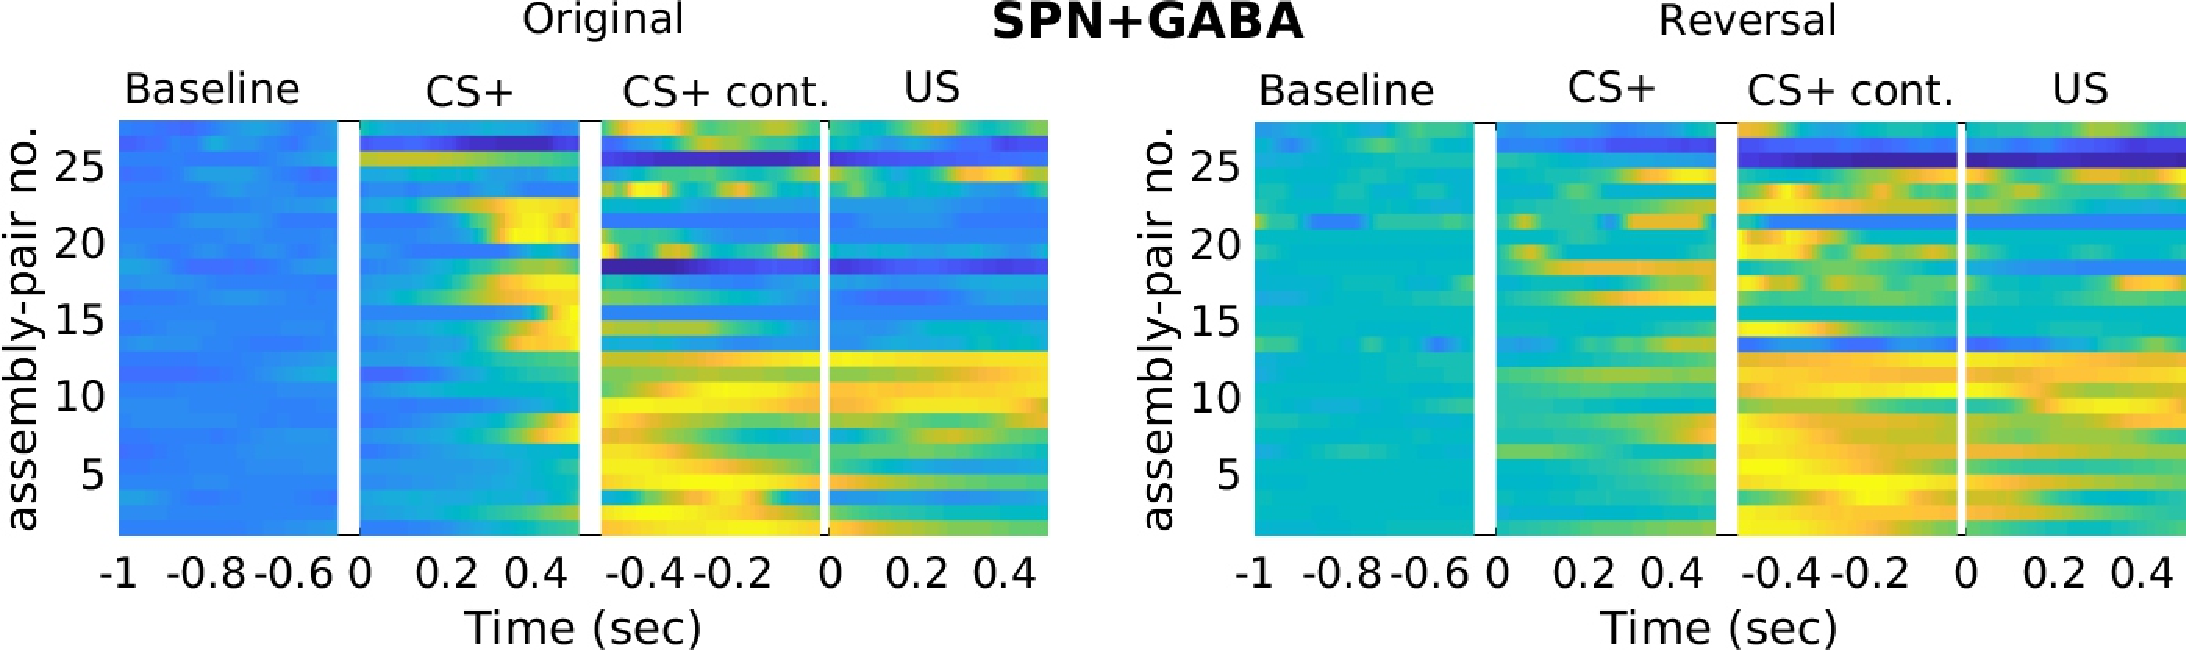
\includegraphics[scale=0.42]{figures/HeatSPN_GABA.pdf}
     
     \vspace{1cm}
     
     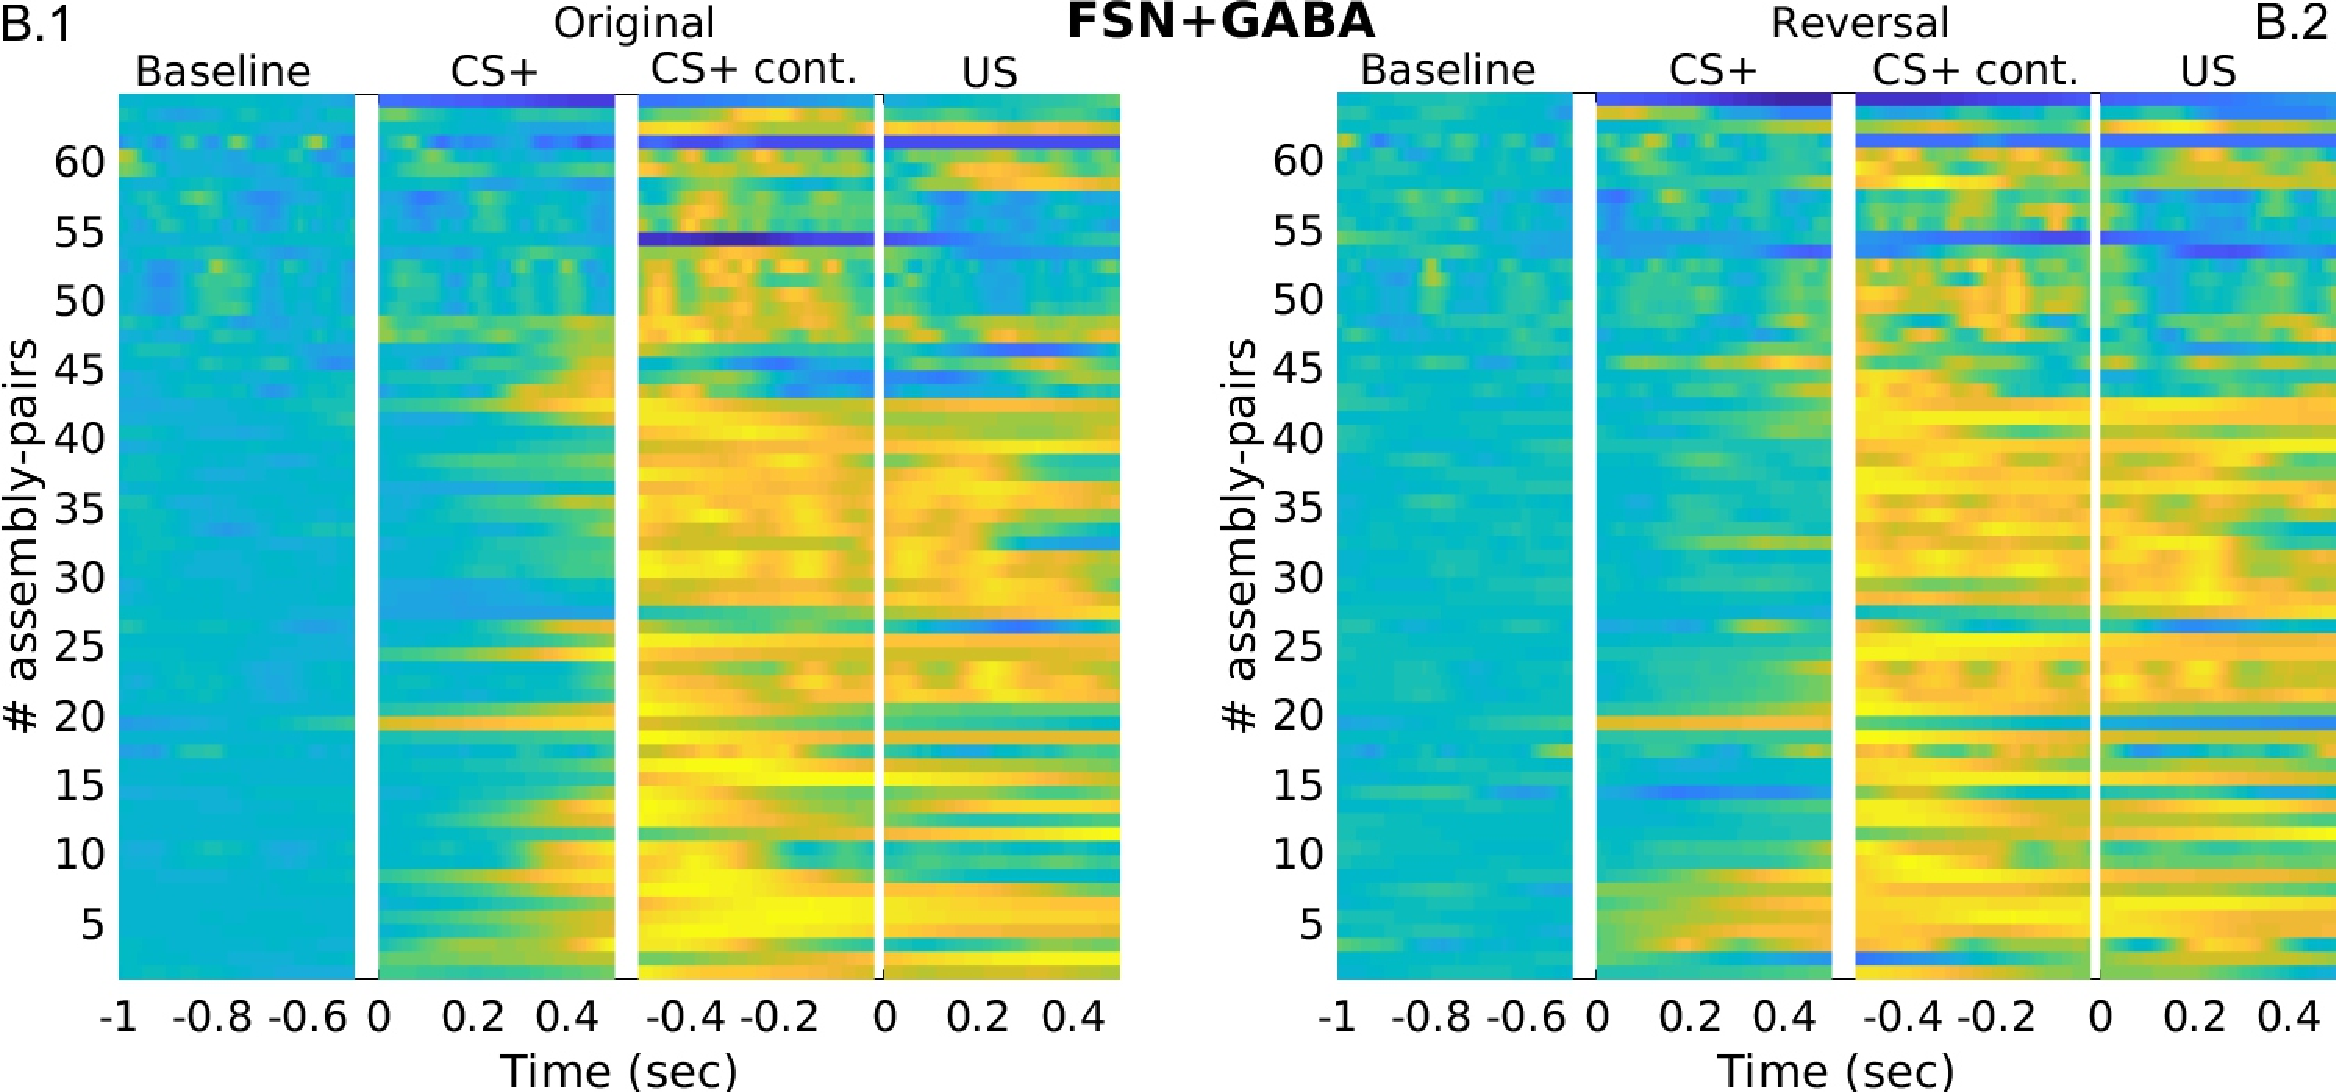
\includegraphics[scale=0.42]{figures/HeatFSN_GABA.pdf}
     \caption{Assembly-pairs tested with Friedman test with significant task related response in original phase. In order: \textbf{Top left:}SPN-GABA assembly-pairs; \textbf{top right:} the same assembly-pairs in the reversal phase. \textbf{Bottom left:} FSN-GABA assembly-pairs in original; \textbf{bottom right:} FSN-GABA assembly-pairs in reversal. The activity was normalized as in eq. \ref{eq:norm} were $\max(I)$ ($\min(I)$) was the absolute maximum (minimum) of assembly-activity among the four windows; the mean of the baseline was subtracted to each assembly. The maximum (minimum) is marked in yellow (deep blue).}
     \label{fig:HeatPairsGaba}
 \end{figure}
 \begin{figure}[H]
    \centering
   % 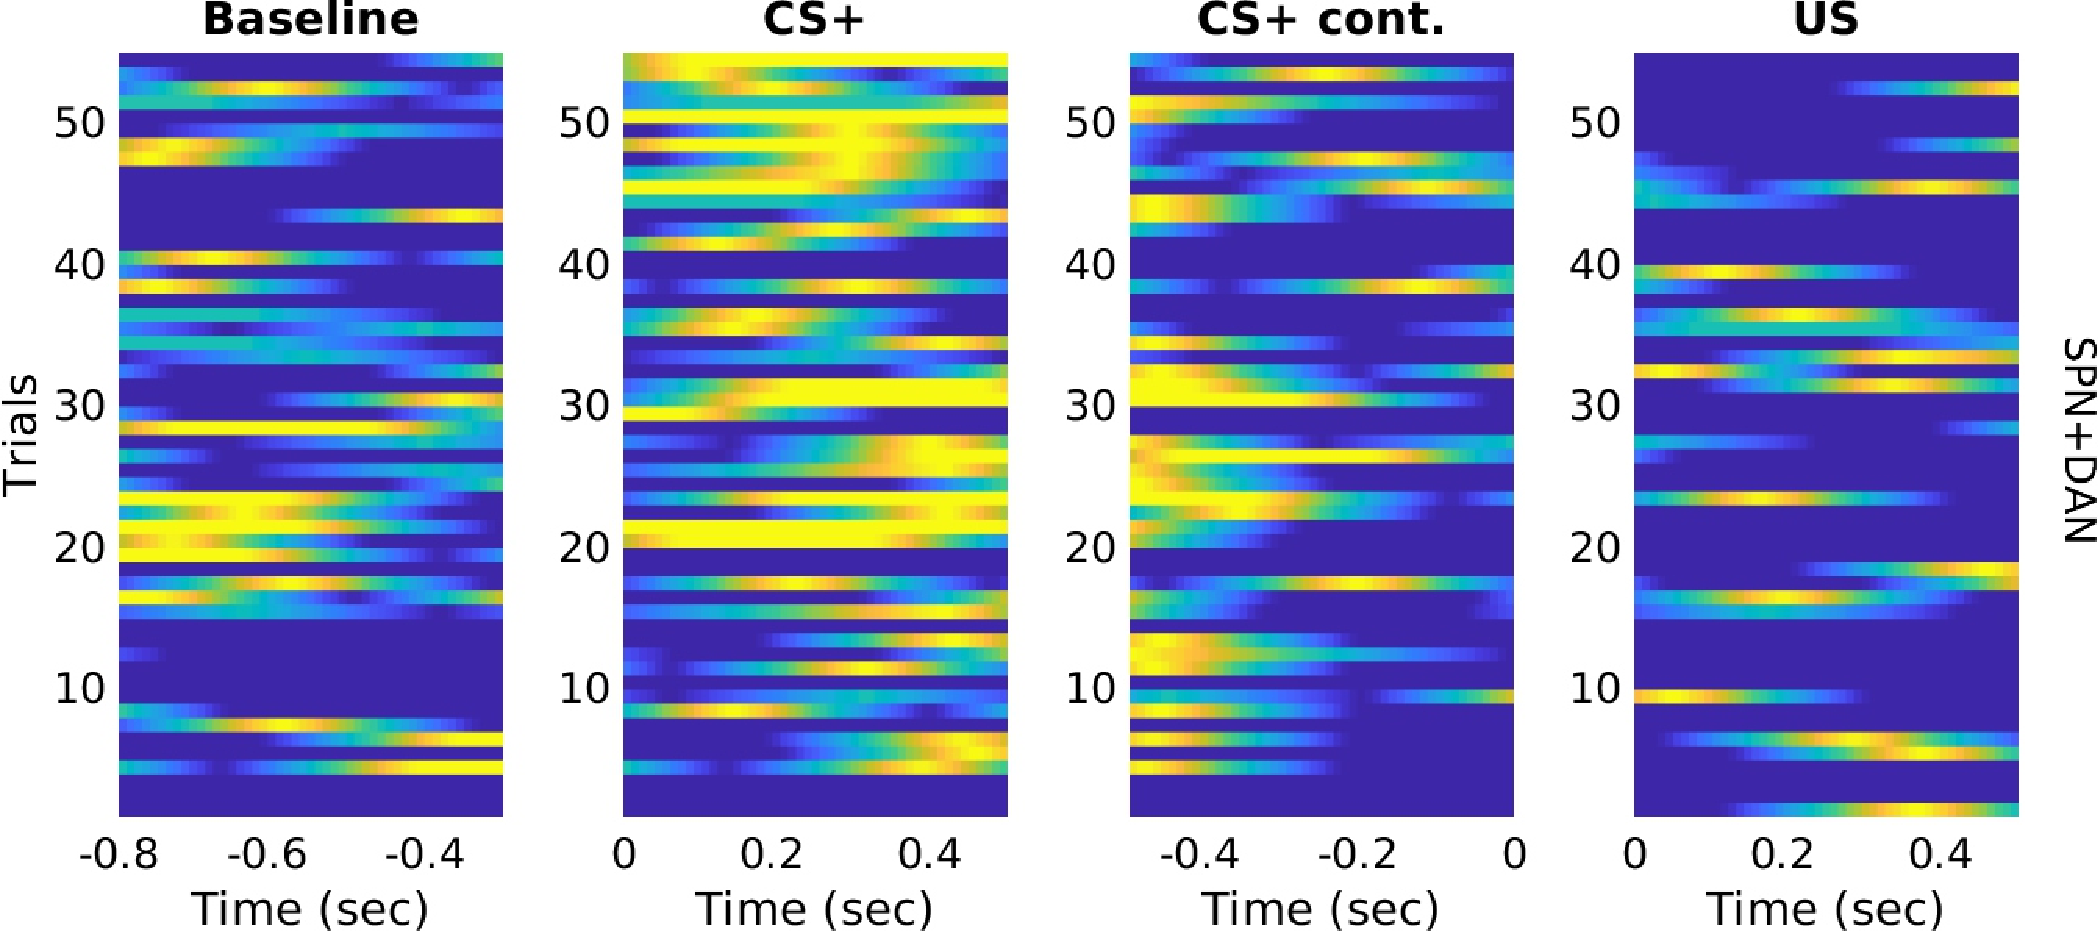
\includegraphics[scale=0.4]{figures/SPN_DANexStim1.pdf}
    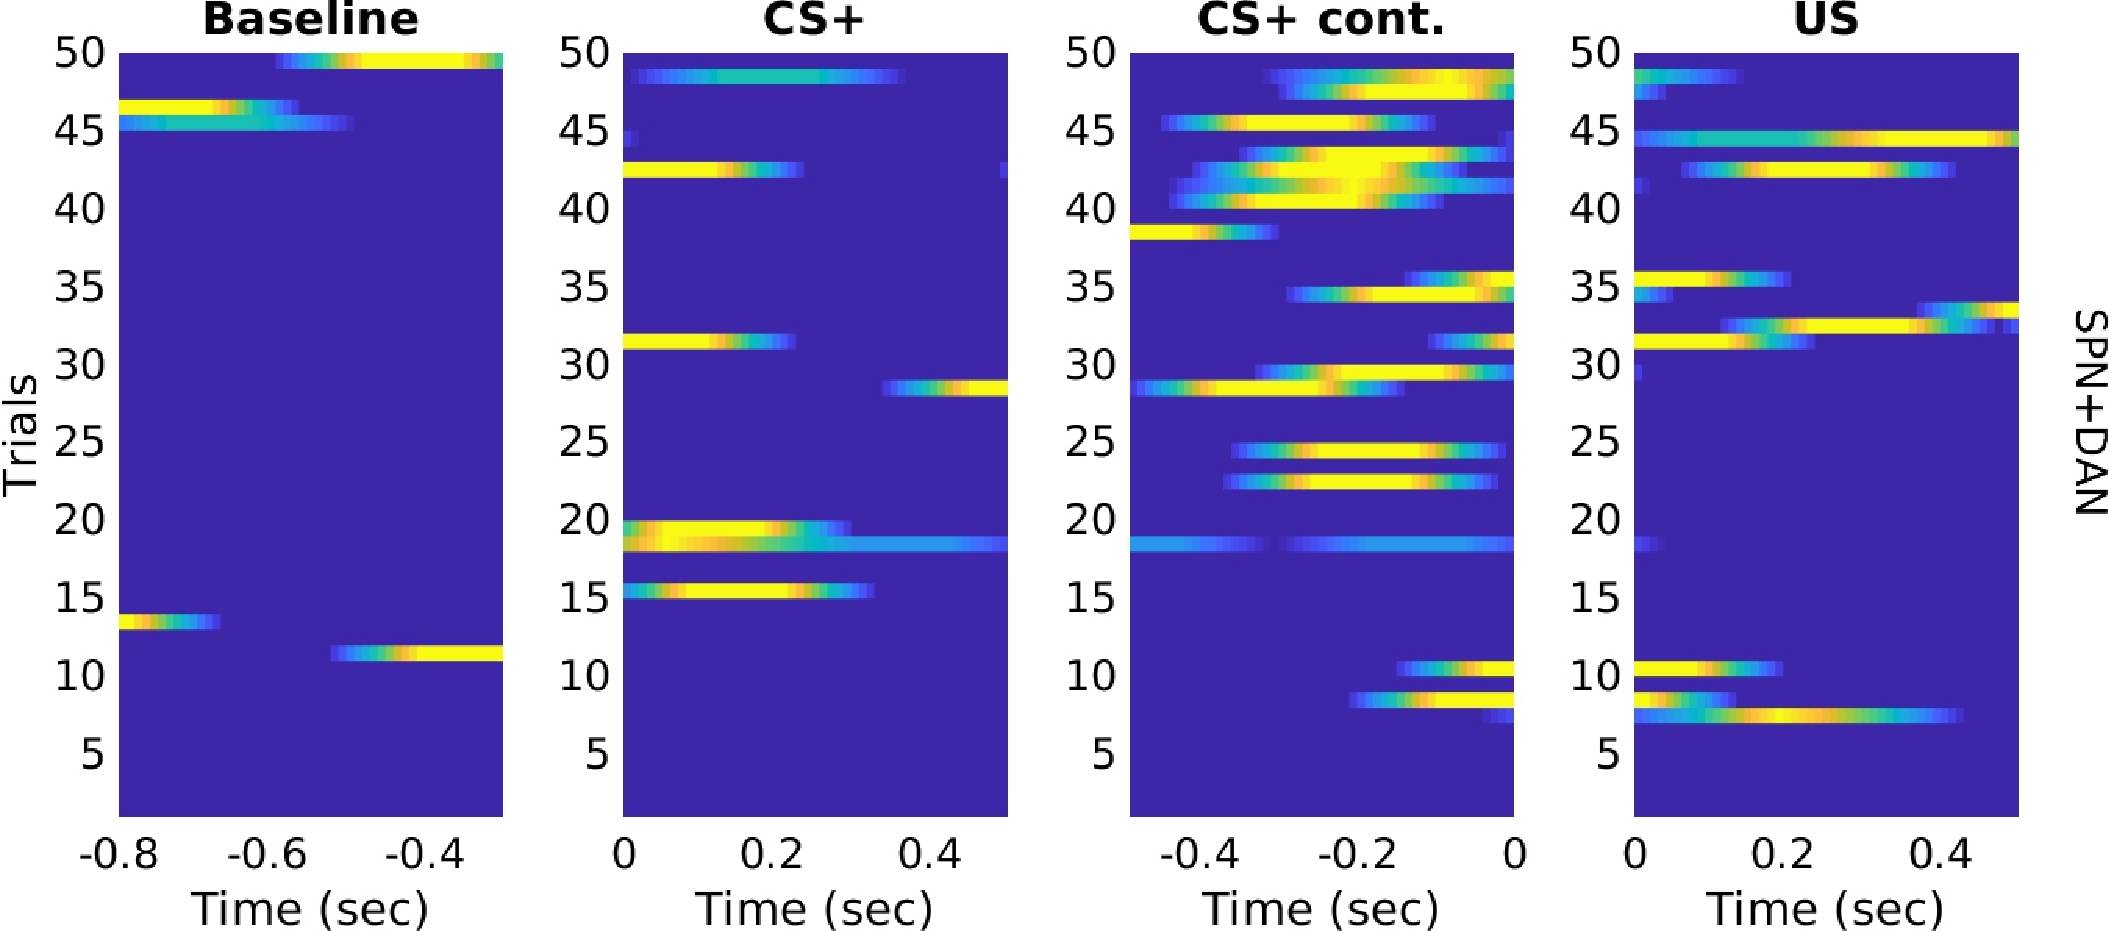
\includegraphics[scale=0.4]{figures/SPN_DANexPreRew.pdf}
    
   \vspace{1cm}
   
   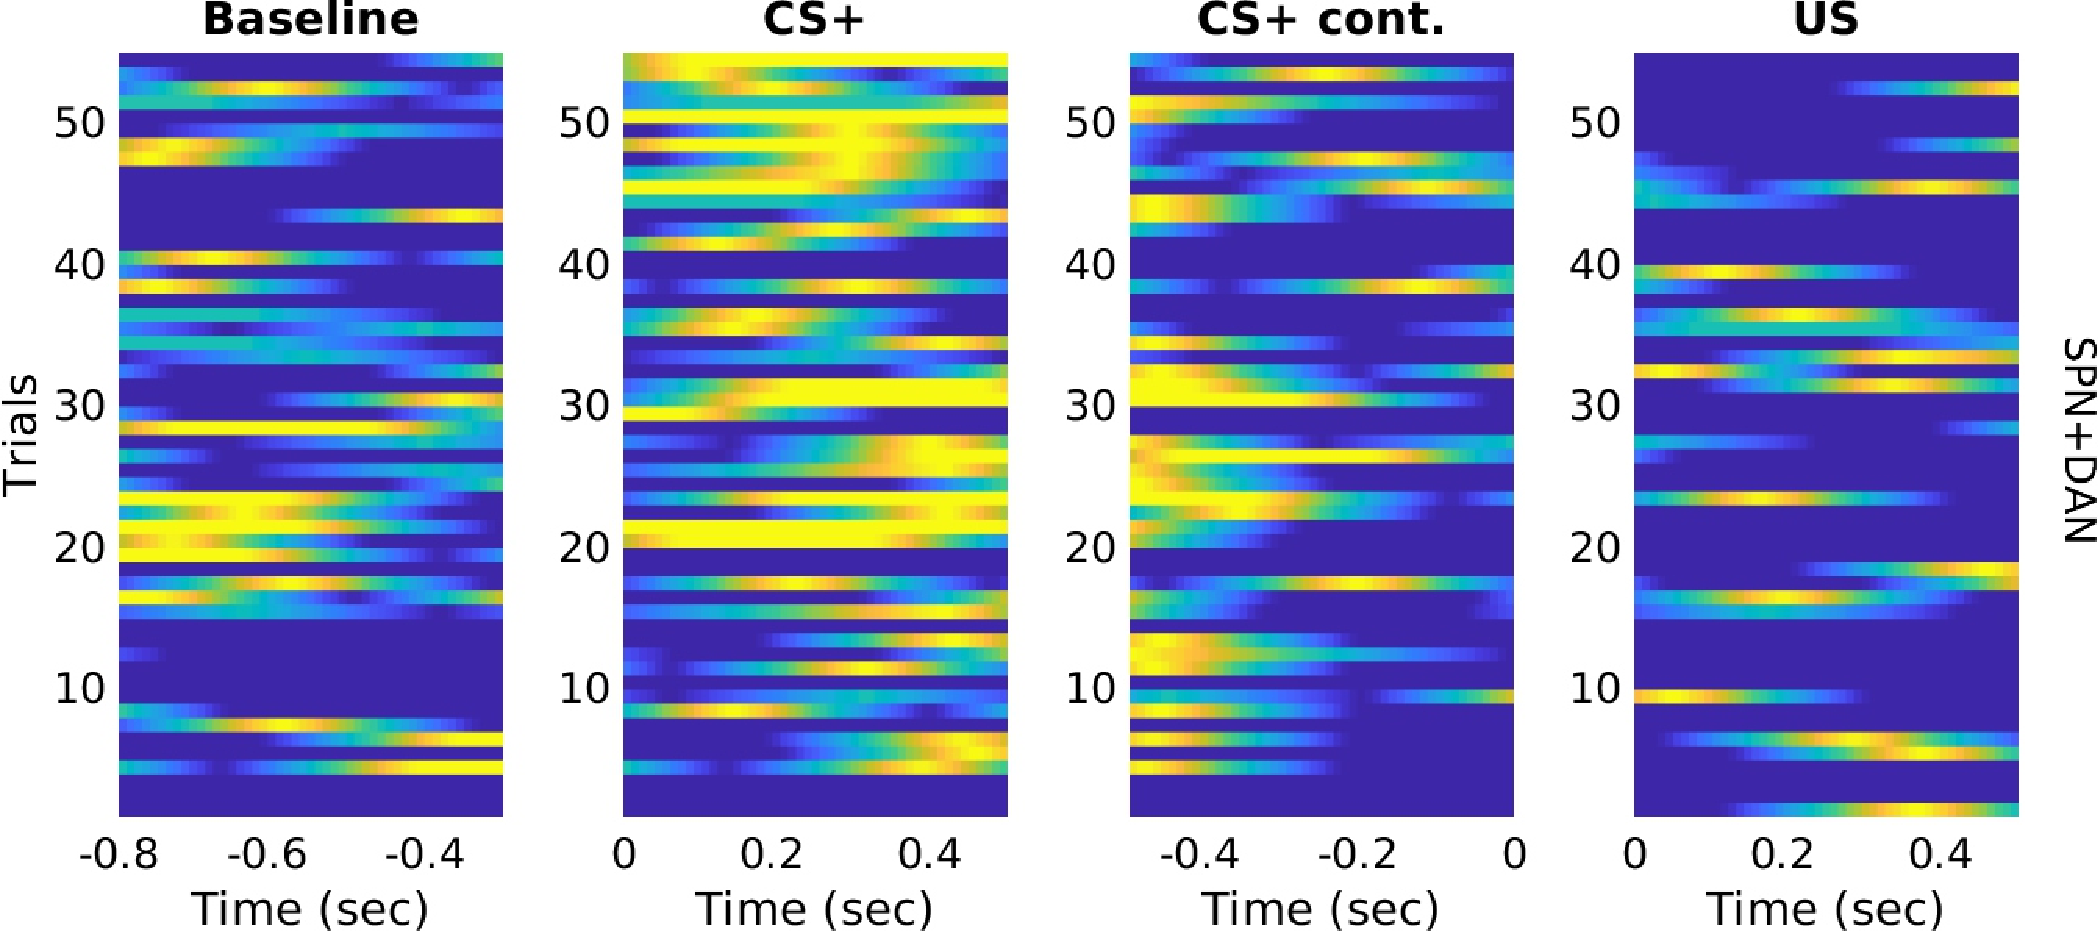
\includegraphics[scale=0.4]{figures/SPN_DANexStim1.pdf}
    \caption{Example of two assembly-pairs significant after the analysis of variance for which the post-hoc test shown that in both cases two groups out of four were significant different, respectively the baseline and the CS+$_{cont}$ window (top) and the baseline and the CS+ window (bottom).}
    \label{fig:SPN_Ex}
\end{figure}
In figure \ref{fig:SPN_Ex} I examined two SPN-DAN pairs closer significant for the Friedman test performed on hit trials (correct trials when the rewarded odor was presented). The post-hoc analysis found for the two assemblies a significant difference between the average activation during the baseline and the CS+$_{cont.}$ window (figure \ref{fig:SPN_Ex}, top) and during the baseline and CS+ (figure \ref{fig:SPN_Ex}, bottom) window, respectively. Interestingly I observed, in significant windows, less assembly-activity in the first trials and more intense assembly-activity in the late trials.\\This dynamical responsiveness resembles typical learning dynamics. In first the trials the mouse is in an explorative period in which the rule of the task has not been learnt yet; while it has been learnt at the end of the original phase. In other words, in the first part of the task the animal is almost always surprised when the reward is delivered, and the expectation of reward is low, while during the second part of the original phase the mouse is able to predict the reward already at the stimulus presentation and the expectation of reward increases when the rewarded stimulus is presented.\\In presence of probabilistic reward the response of dopamine units is peaked at the reward time when the probability to get the reward is low and is instead peaked at stimulus presentation when the probability to get the reward is high (\cite{Schultz1992}, \cite{Schultz} \cite{Fiorillo}). VS neurons instead show a tonic response with the stimulus presentation and their neuronal activity is modified when the subject learns to predict future rewards from sensory cues (\cite{Pagnoni}, \cite{Schultz2000}, \cite{Radua}).\\Thus if an assembly-pair codes for reward prediction error, then the activity should be intense during the presentation of the rewarded stimulus only in the last part of the task-phase. On the contrary, in pairs significant at retrieval (US) one would expect intense activity in first trials, related to the surprise to have the reward, and less activation in the second part of task, when the animal is more certain about the reward. I will examine these learning transitions revealed in the variability across trials in \hyperref[sec:CorrRL]{~Chapter \ref*{sec:CorrRL}}.\\The two examples in figure \ref{fig:SPN_Ex} show that some assembly-pairs are implicated in the learning dynamic, by analysing systematically the assembly activity with respect to the animal behavior, one can understand how many of them are involved in the learning dynamic and which functions they express. Assuming that a good portion of assembly-pairs show a learning dynamic, one would ask: are they all involved specifically in prediction error computation? Do they compute differently the prediction error signal depending on their underlying units? Reward prediction error signals in DAN are formed by two components (\cite{Tobler2003}, \cite{Nomoto2010}, \cite{Fiorillo2013}, \cite{Schultz2016}): the first component consists in an early activation due to an unselective response to a large variety of unpredicted events including the potentially rewarded stimuli, that are however in this phase only detected, and only later identified and valuated.\\The detection component evolves then into the second component, also called main component, which reflects the evolving neuronal processing that is required to evaluate and appreciate the stimulus (see figure \ref{fig:probDopamine} in \hyperref[chap:Introduction]{Chapter~\ref*{chap:Introduction}}). This latter component is the biological implementations of reward prediction error term present in reinforcement learning models.\\Despite clear evidence for DAN involvement in prediction coding, it is hard to identify how these signals are encoded by the larger circuit. This work was aimed to prove that the specificity of different components coding emerges in the assembly-pairs activity because different interactions convey different aspects of the prediction error coding. DAN exhibit homogeneous response across the population in order to ensure a robust and efficient coding (\cite{UchidaDop}), which could become specific through distinct VS interactions. The learning functions would then be, rather circuit specific than cell-types-specific.\\In light of the considerations above and based on the activation patterns shown in figure \ref{fig:HeatPairsDan}, one can assume that SPN-DAN assembly-pairs are thus good candidates for prediction coding (figure \ref{fig:HeatPairsDan}, top). Conversely the early activation to the stimulus of FSN-DAN pairs (figure \ref{fig:HeatPairsDan}, bottom) may suggest that these assemblies are involved in stimulus salience, that reflects the detection component of RPE. One hypothesis could be that the detection component of prediction error is formed in FSN-DAN assembly-pairs, which evolves in the identification and valuation coding through the SPN-DAN circuit.
Those consideration will be discussed in detail in \hyperref[sec:FalseAlCorrRej]{Section~\ref*{sec:FalseAlCorrRej}}, as well in \hyperref[sec:CorrRL]{Chapter~\ref*{sec:CorrRL}}, and \hyperref[sec:Regression]{Chapter~\ref*{sec:Regression}}.\\Since I specifically wanted to investigate how prediction signals were formed in VS-VTA interaction, I focused only on the interregional assembly-pairs with DAN in the subsequent analysis.\\
\section{Hit, False Alarm and Correct Rejection Trials}
\label{sec:FalseAlCorrRej}
When the animal receives unexpectedly reward, DAN fire a burst of action potentials. If a sensory stimulus reliably predicts reward, however, DAN decrease their response to reward, and instead burst to the stimulus, and finally if an expected reward is omitted, DAN pause their firing at the time they usually receive reward (\cite{Schultz1997}, \cite{Wenzel}, \cite{Fiorillo2013b}, \cite{Schultz2015}).\\The comparison between Hit, False Alarm and Correct Rejection is interesting because I expected different VS-VTA assembly-pair activations in relation with reward prediction and reward occurrence.\\I assumed that assembly-pair task related patterns reflect the predictive coding of underlying units, furthermore I expected that assembly analysis could reveal how the prediction signal is formed in VS-VTA circuit, question that is in fact still discussed and unclear (\cite{Takahashi2016}, \cite{Saunders2018}).\\If the hypothesis of a circuit specialized code is true, I should observe differences in activity patterns of VS-VTA assembly-pairs composed by DAN with different cell-types in VS. In the previous session the two sequential components of neuronal response were introduced, the first called detection, and the main component, called identification and valuation. It was suggested as well that sharp assembly-pairs FSN-DAN encode a generic detection of the stimulus, whereas SPN-DAN assembly pairs, characterized by broader response could encode the valuation, that is the component associated to the prediction error in reinforcement learning models.\\In the previous section I examined the response of assembly-pairs in Hit trials. Hit trials are trials in which the odor was followed by reward and the mouse went for the reward. I had identified assembly-pairs with significant task-related activation.\\In the same way, I had analysed the assembly-pairs task-related response for False Alarm trials (unrewarded odor, the mouse went for reward) and Correct Rejection trials (unrewarded odor, the mouse did not lick). The three windows of interest were set up for these trials types in the following ways: in False Alarm trials those windows were called CS-, CS-$_{cont.}$, 3rd Lick. The CS- window, analogously to the CS+ in Hit trials, was a time interval of 0.5 $sec$ starting from the stimulus onset (unrewarded in this case); the CS-$_{cont.}$ and 3rd Lick were respectively the time intervals, again 0.5 $sec$ long, immediately before and after the expected reward.\\I used the following assumption to establish the expected reward time in unrewarded trials: since in cases in which the rewarded odor was presented the mouse had to lick at least two or three times (depending on the paradigm) to get the reward, I assumed the animal to expect the reward after the second or the third lick (depending on the current paradigm) even when the odor was unrewarded.\\In Correct Rejection trials, CS- and CS-$_{cont.}$ intervals were defined similar to the False Alarm trials. In this case the animal did not expect the reward, however, I analysed the assembly-pairs activity also in the $"$hypothetical reward$"$ window for comparison. I used as $"$hypothetical reward$"$ time, the average reward time obtained from Hit trials, to compare the assembly-pairs activity before and after the $"$hypothetical reward$"$ time with the activity before and after the reward time (Hit trials) or the expected reward time (False Alarm trials).\\\\\\\\
\subsection{SPN-DAN assembly-pairs}
Figure \ref{fig:HeatSPN_DANComp} shows SPN-DAN pairs task-related activity in Hit, False Alarm and Correct Rejection trials. In Hit trials the assembly-pairs activation was lead mainly by the rewarded odor. A good portion of assemblies were significantly active only in CS+ ($~ 45\%$), fewer were continuously active in CS+ and CS+$_{cont}$ ($~17\%$) and only $~5\%$ of assembly were active from the stimulus onset to the time including the retrieval. Finally I note that a relative small fraction was active around the reward time in CS+$_{cont}$ and US ($~ 14\%$).\\SPN-DAN pairs were less activated at the stimulus onset in False Alarm trials than in Hit trials. Indeed, in False Alarm trials the animal was unsure about the stimulus received and not able to predict the reward-outcome. While in Hit trials, the animal was more confident\footnote{I explain the distinction between the early and the final stage of the task in \hyperref[chap:RLModel]{Chapter ~\ref*{chap:RLModel}}} about the outcome to be received, and thus, being able to predict the reward, reacted to the conditioned stimulus, in agreement with the prediction error signals.\\Much less SPN-DAN assembly-pairs show significant task-related response in Correct Rejection trials than in Hit trials suggesting that SPN-DAN assembly-pairs preferentially code for the rewarded odor. Finally figure \ref{fig:SD_HitCorrComp} shows the comparison of assembly-pair activity in Hit and Correct Rejection trials, for those assembly-pairs significant in Hit trials. While the rewarded odor lead the SPN-DAN pairs activity, those assembly-pairs were not equally activated by the unrewarded odor. This result confirmed that SPN-DAN pairs were selective for the rewarded odor. Figure \ref{fig:Overlap} shows which fraction of the assemblies significant in the CS+ window of the Hit trials (rewarded odor) was also significant in the CS- window of Correct Rejection trials (unrewarded odor). Of SPN-DAN assembly-pairs only the $12\%$ showed a stimulus-related activity for both rewarded and unrewarded odors. On the contrary a large fraction of FSN-DAN assembly-pairs ($68\%$) unspecifically responded to both stimuli. These results indicated that FSN-DAN pairs unspecifically respond to the stimulus.\\\\\\\\\\\\\\\\\\\\\\\\\\\\\\\\\\\\\\
\begin{figure}[H]
\centering
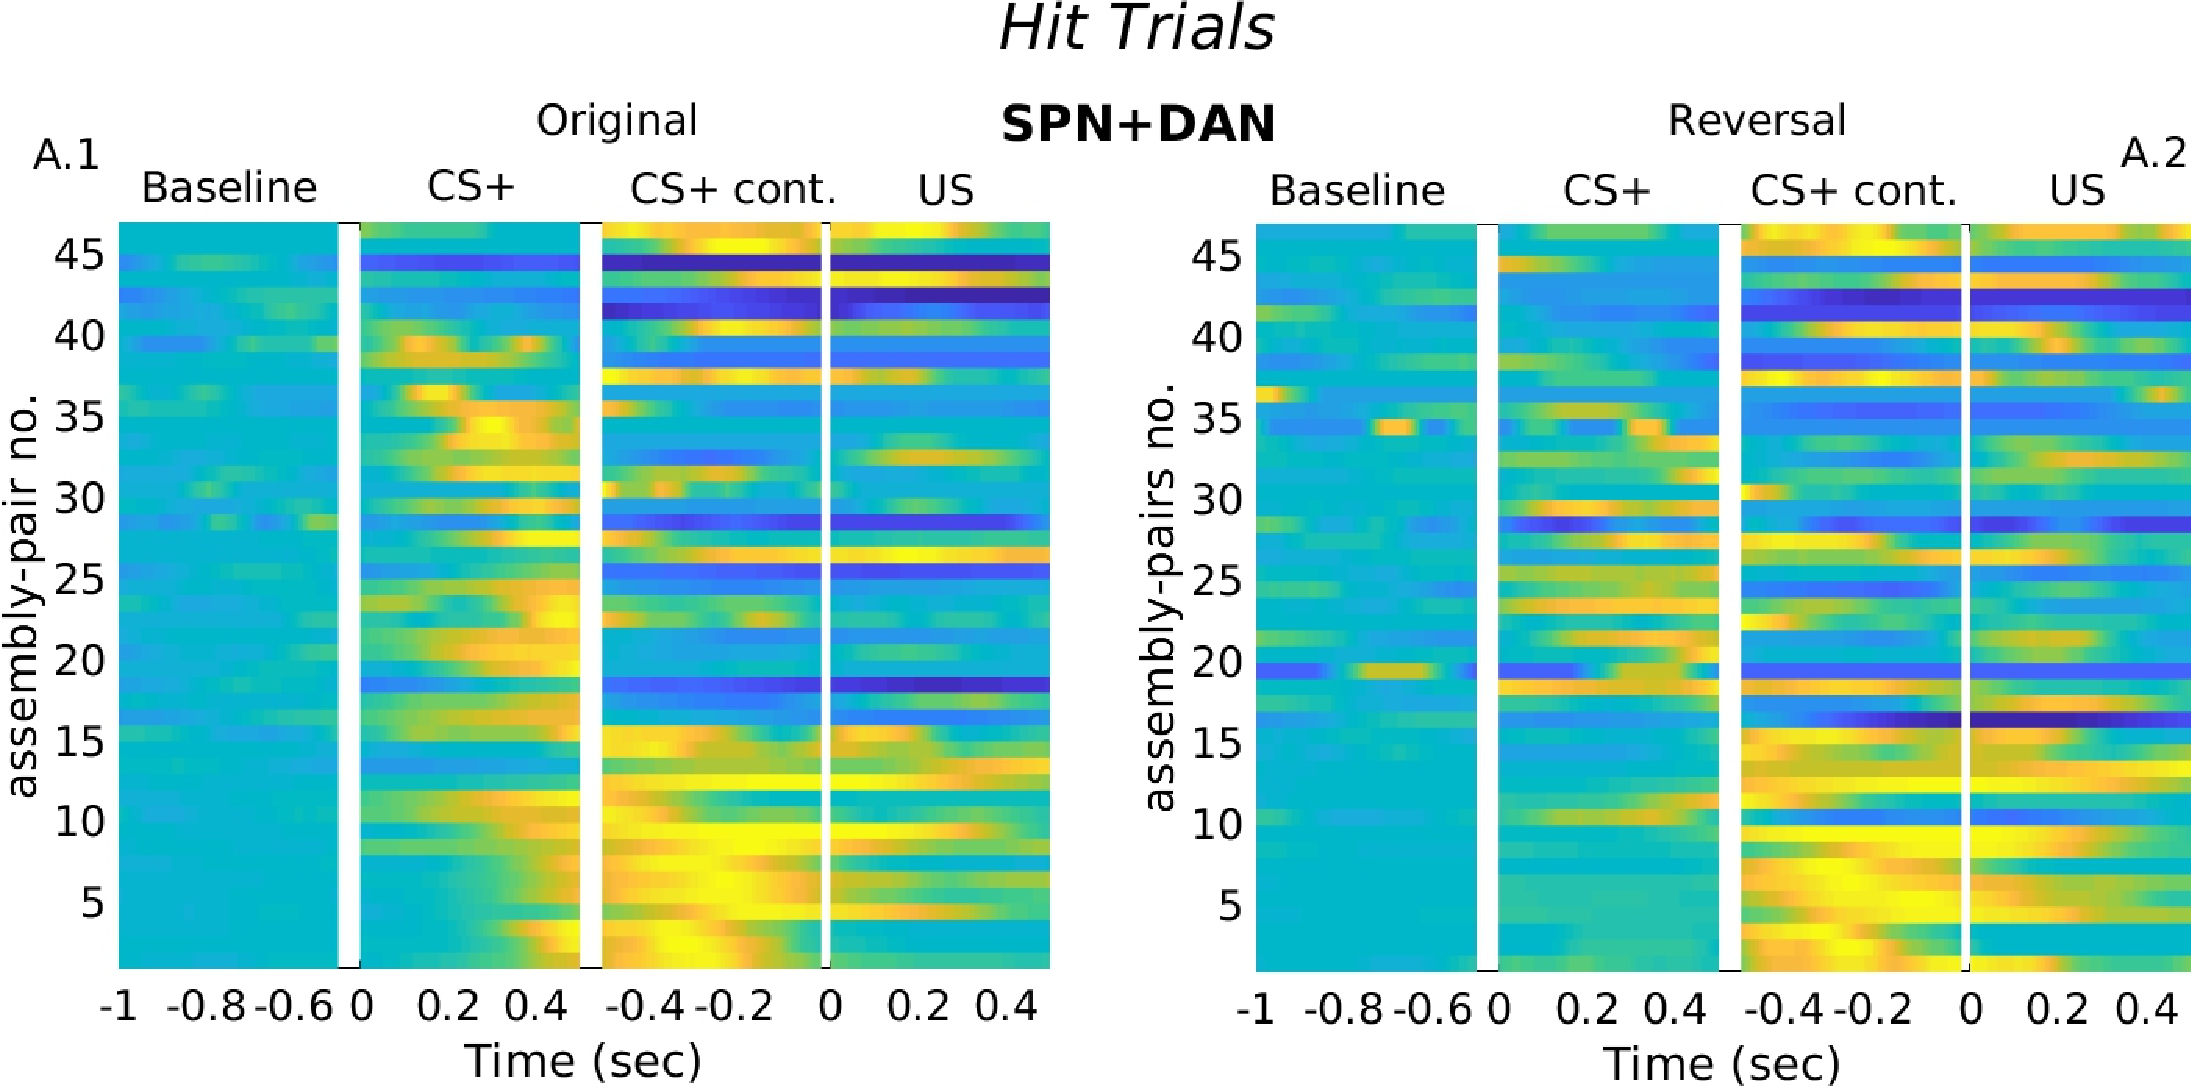
\includegraphics[scale=0.4]{figures/SPN_DANHit.pdf}

\vspace{0.5cm}

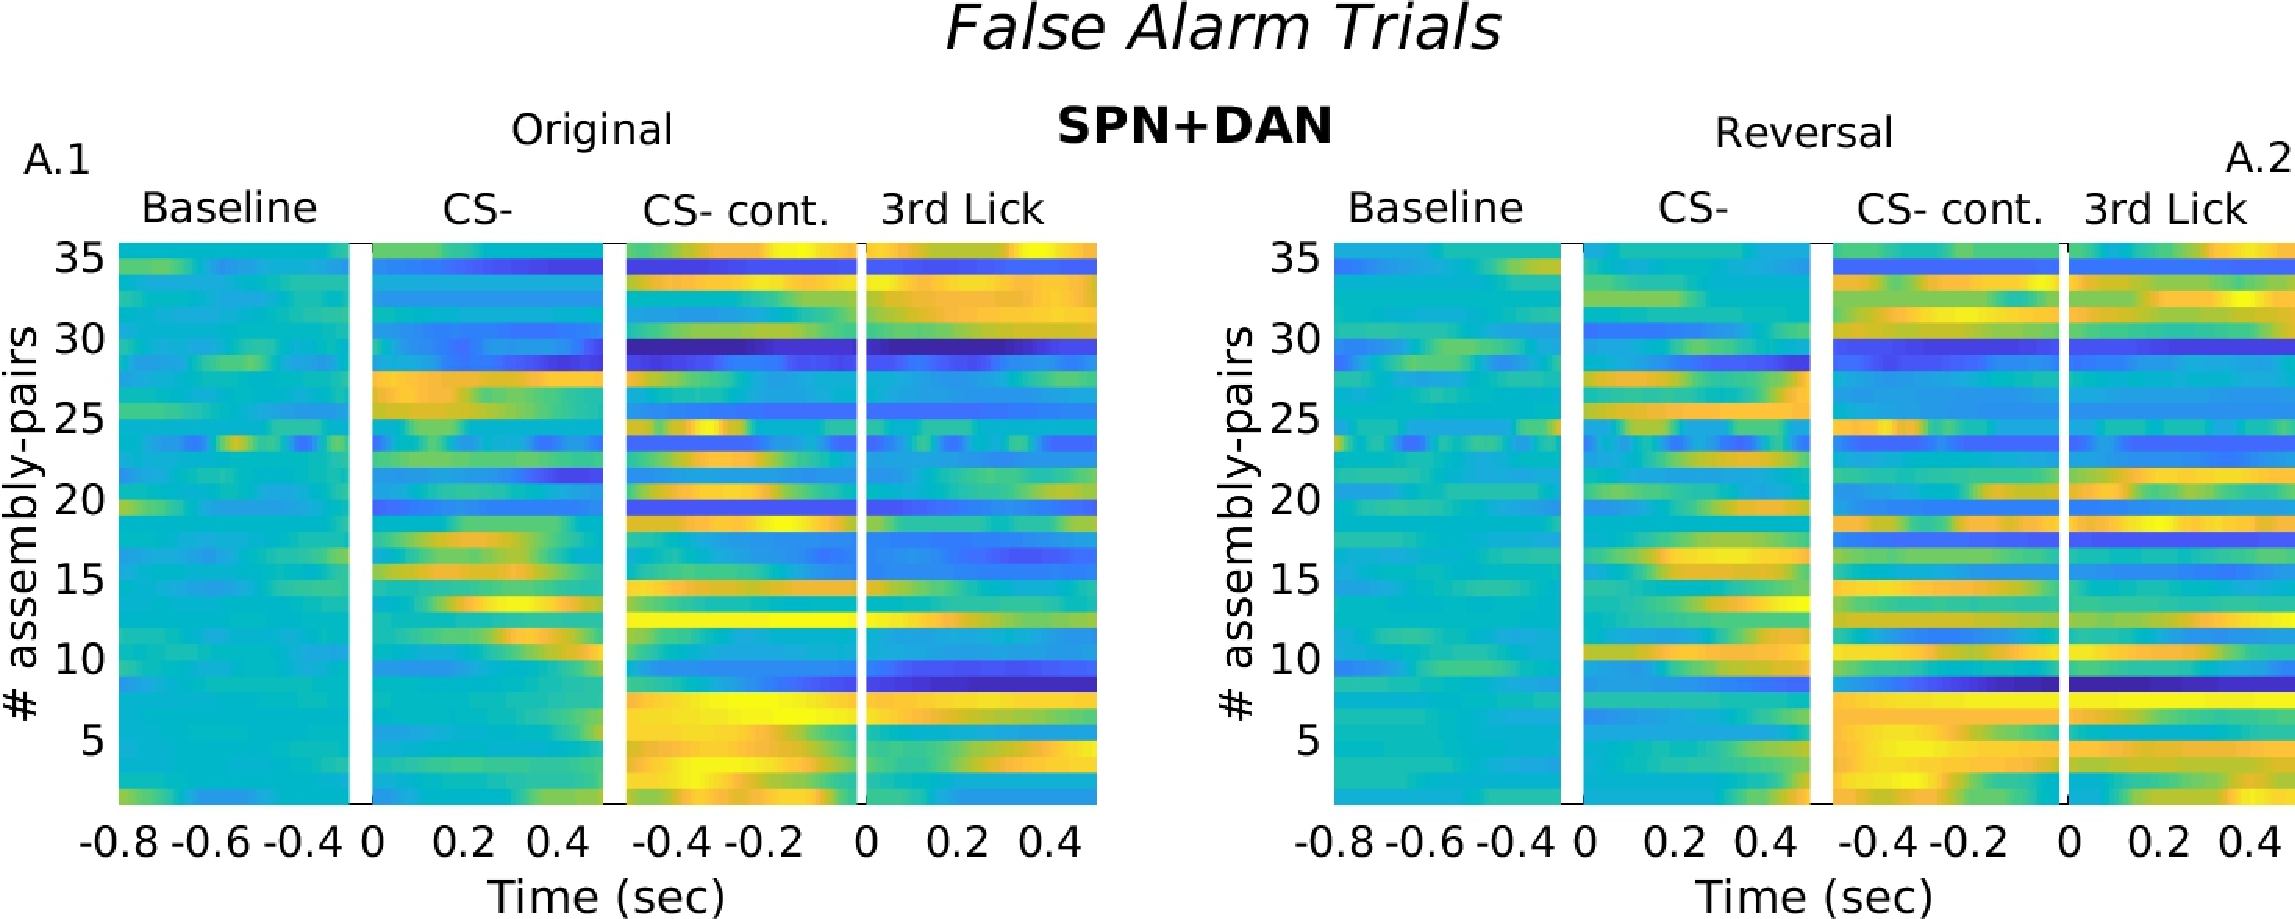
\includegraphics[scale=0.4]{figures/HeatFA_SPN_DAN.pdf}

\vspace{0.5cm}

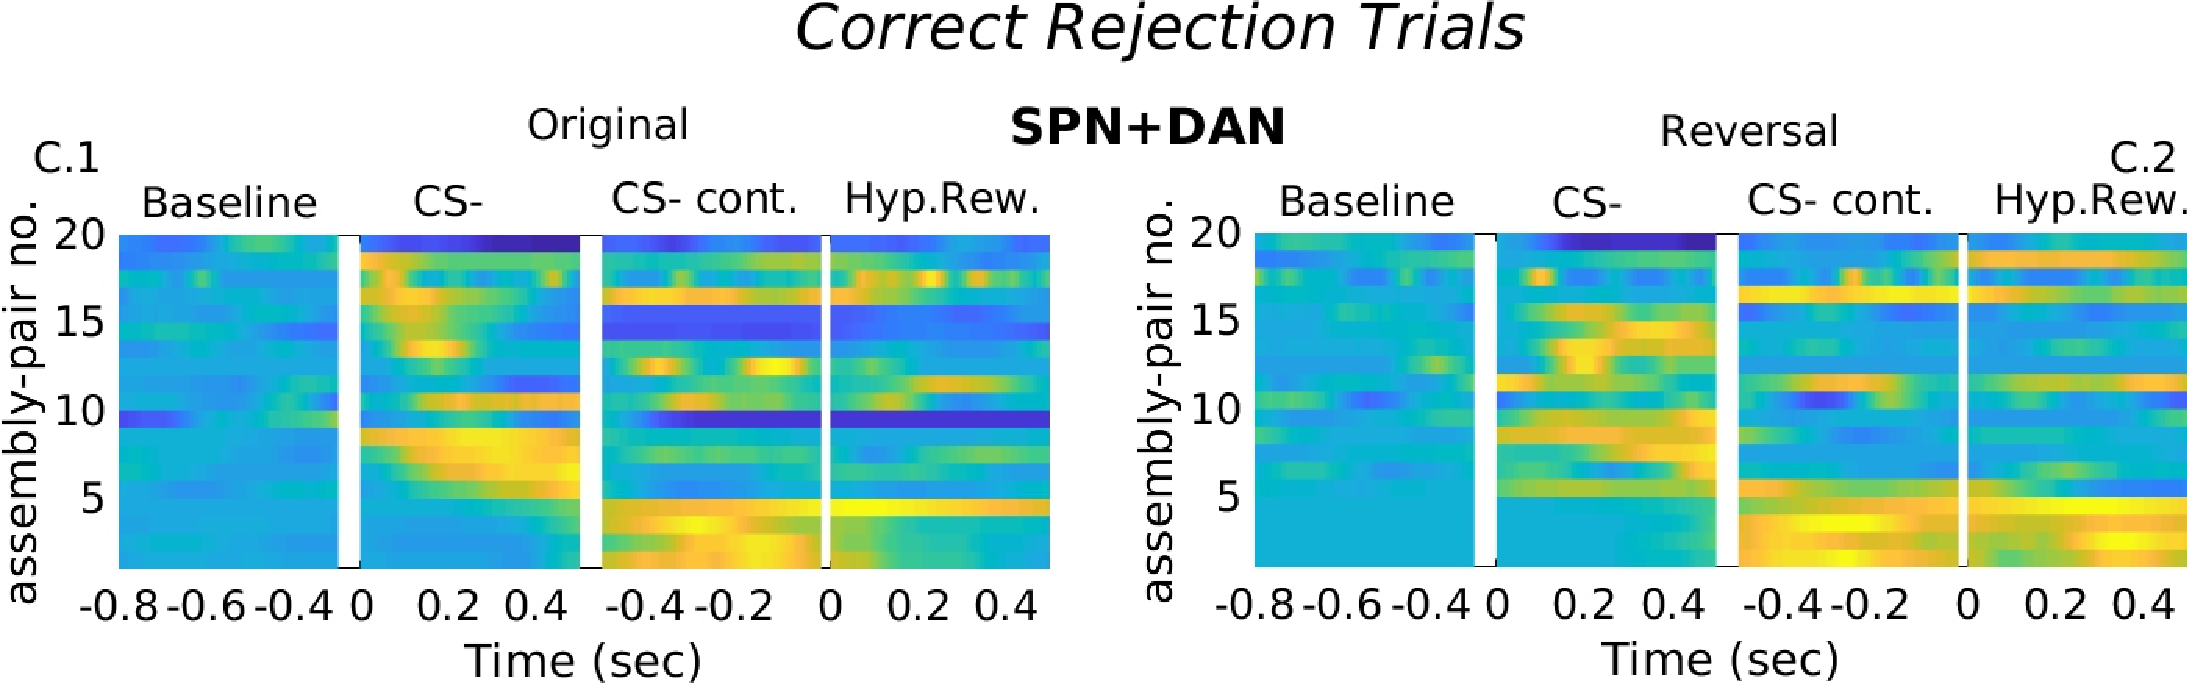
\includegraphics[scale=0.4]{figures/HeatCR_SPN_DAN.pdf}
\caption{Heat map of significant activation of SPN-DAN assembly-pairs (Friedman test) in three trial segments (Hit, False Alarm and Correct Rejection). In Correct Rejection trials much less assembly-pairs were significant. SPN-DAN assembly-pairs preferentially coded for the rewarded odor. After applying the normalization as in eq. \ref{eq:norm} were $\max(I)$ ($\min(I)$) was the absolute maximum (minimum) of assembly-activity among the four windows, the mean of the baseline was subtracted to each assembly.}
\label{fig:HeatSPN_DANComp}
\end{figure}
\begin{figure}[H]
\centering
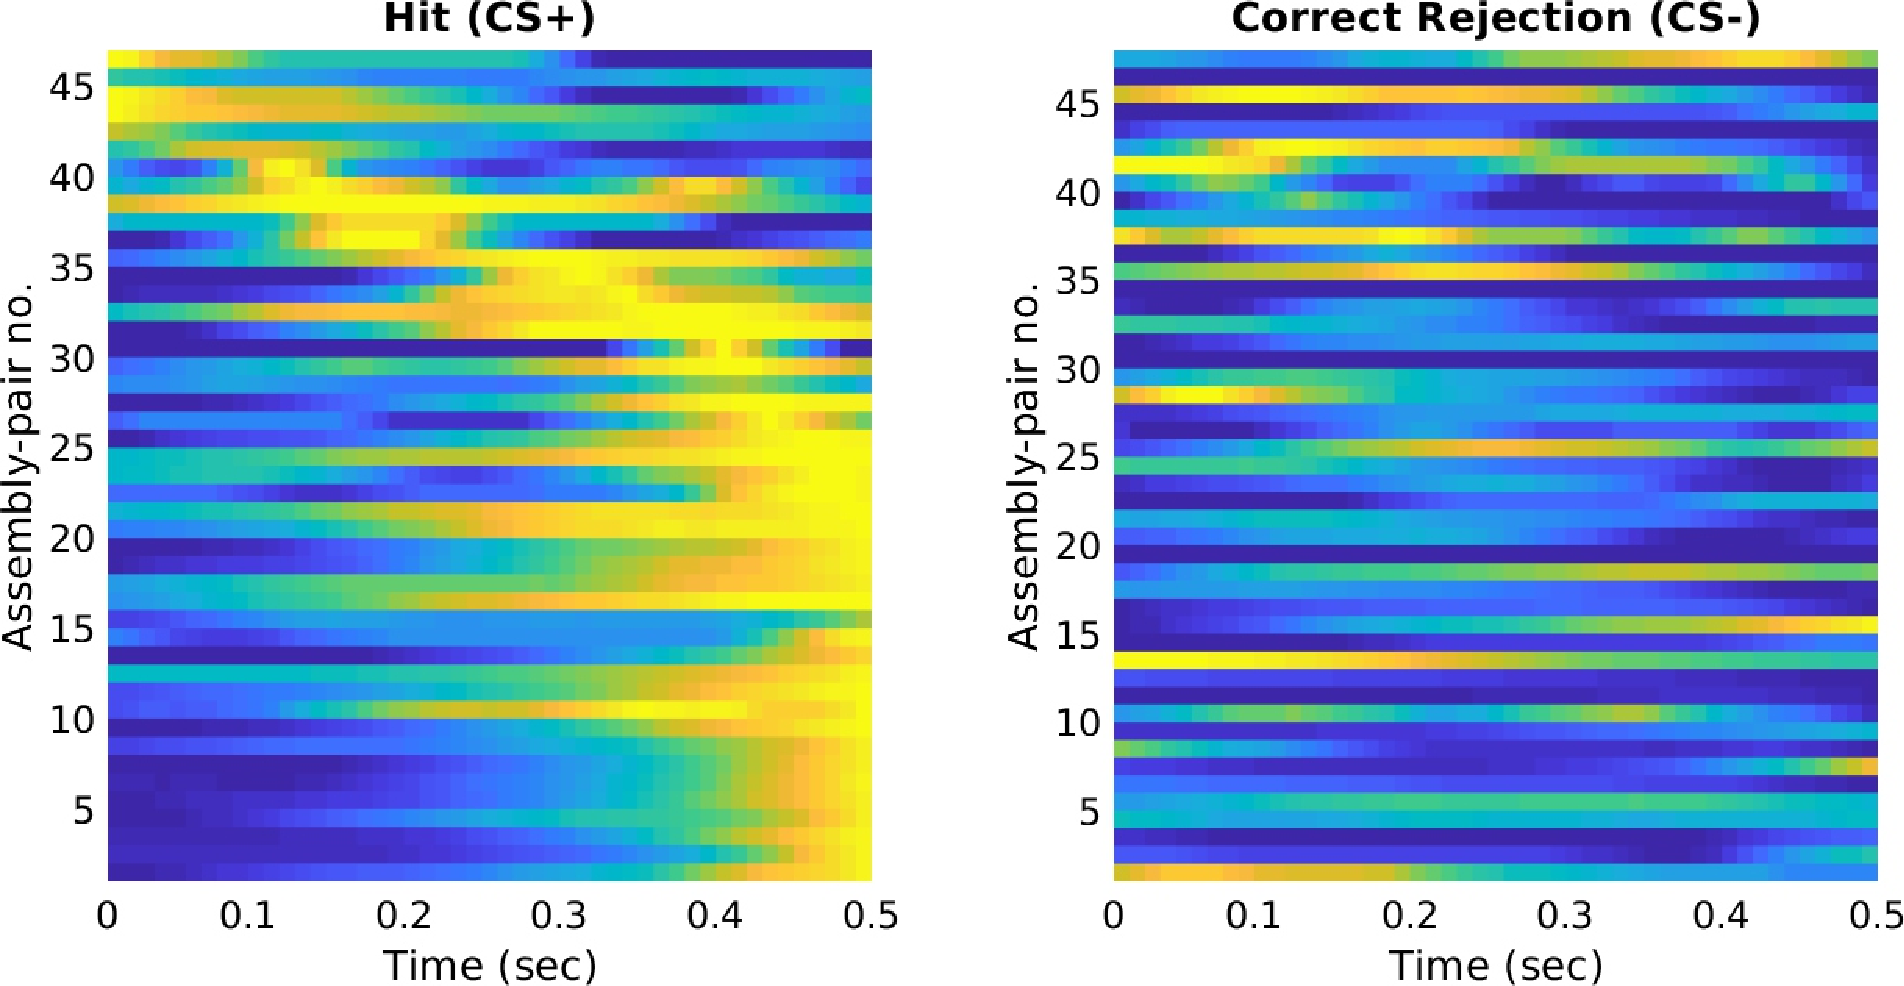
\includegraphics[scale=0.5]{figures/SD_HitCorrRejComp.pdf}
\caption{Heat map of SPN-DAN assembly-pairs significant in Hit trials (Friedman test in Hit trials), represented in Hit and Correct Rejection trials. Here is shown the activity in the window after the stimulus onset (CS+ in Hit trials and CS- in Correct Rejection trials). The activity of each assembly was normalized as in eq.\ref{eq:norm} were $\max(I)$ ($\min(I)$) was the absolute maximum (minimum) of assembly-activity between the two windows.}
\label{fig:SD_HitCorrComp}
\end{figure}

\vspace{1cm}

\begin{figure}[H]
\centering
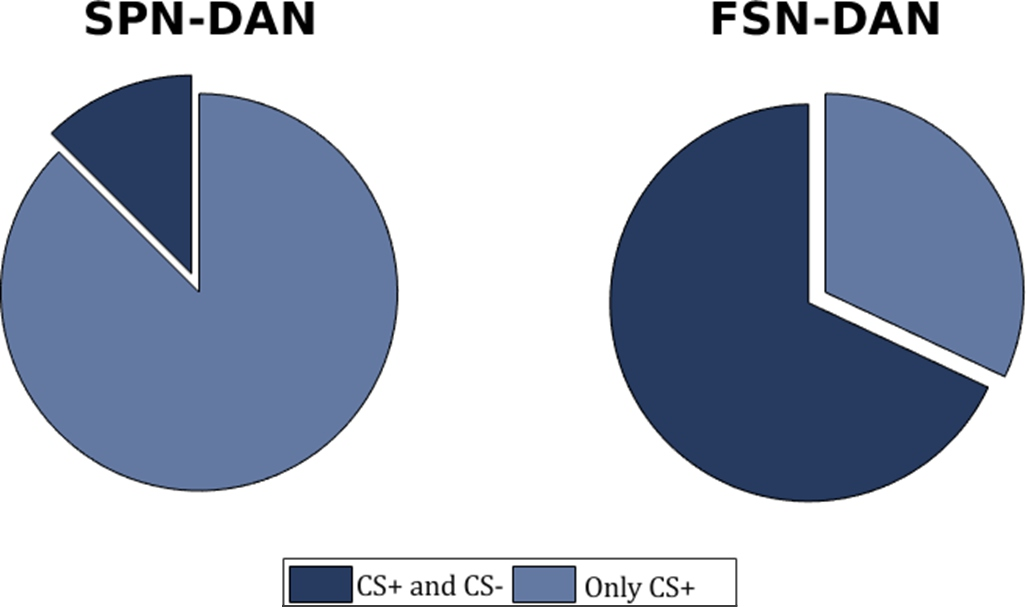
\includegraphics[scale=0.65]{figures/HItCorrRejPieOverlapSD_FD.pdf}
\caption{Assembly-pairs significant in Hit trials divided in the fractions significant during CS+ only in Hit trials and in Hit and Correct Rejection trials. \textbf{Left:} SPN-DAN assembly-pairs. \textbf{Right:} FSN-DAN assembly-pairs.}
\label{fig:Overlap}
\end{figure}

\subsection{FSN-DAN pairs}
FSN-DAN assembly-pair activity patterns were more diverse in their task dependent activation patterns, consistent with the hypothesis that they are unselective to the stimulus type and multisensory in response. In Hit trials (figure \ref{fig:HeatFSN_DANComp}, panels A.1, A.2) the stimulus (CS+) led an early activation, which could be associated to the detection of the signal (see discussion \hyperref[chap:Conclusion]{~Chapter\ref*{chap:Conclusion}}). In Hit trials more than $50\%$ of FSN-DAN pairs were phasically activate during the retrieval (US), suggesting that those pairs are not involved in the prediction of the reward. The phasic activation could correspond a lick-related activity or a hedonic signal. In False Alarm and Correct rejection trials (figure \ref{fig:HeatFSN_DANComp}, panels B.1, B.2, C.1, C.2) the stimulus, unrewarded in this case (CS-), led to the activation of the majority of FSN-DAN pairs, both in the original and reversal phase. As shown in figure \ref{fig:Overlap} the identities of those pairs activated by the stimulus in Hit trials overlapped most of the time with those active in Correct Rejection trials, proving that the activation to the stimulus is not a reward related predictive signal. This rather unspecific salience could correspond general salience signal and hedonic signals as one may expect for VP units.\\I note that of FSN-DAN pairs were also sparsely inhibited; particularly in False Alarm and Correct Rejection trials. This inhibition could be again related to motivational factors, such as $"$disappointment$"$. 
 \begin{largefigure}[17pt]
 \centering
 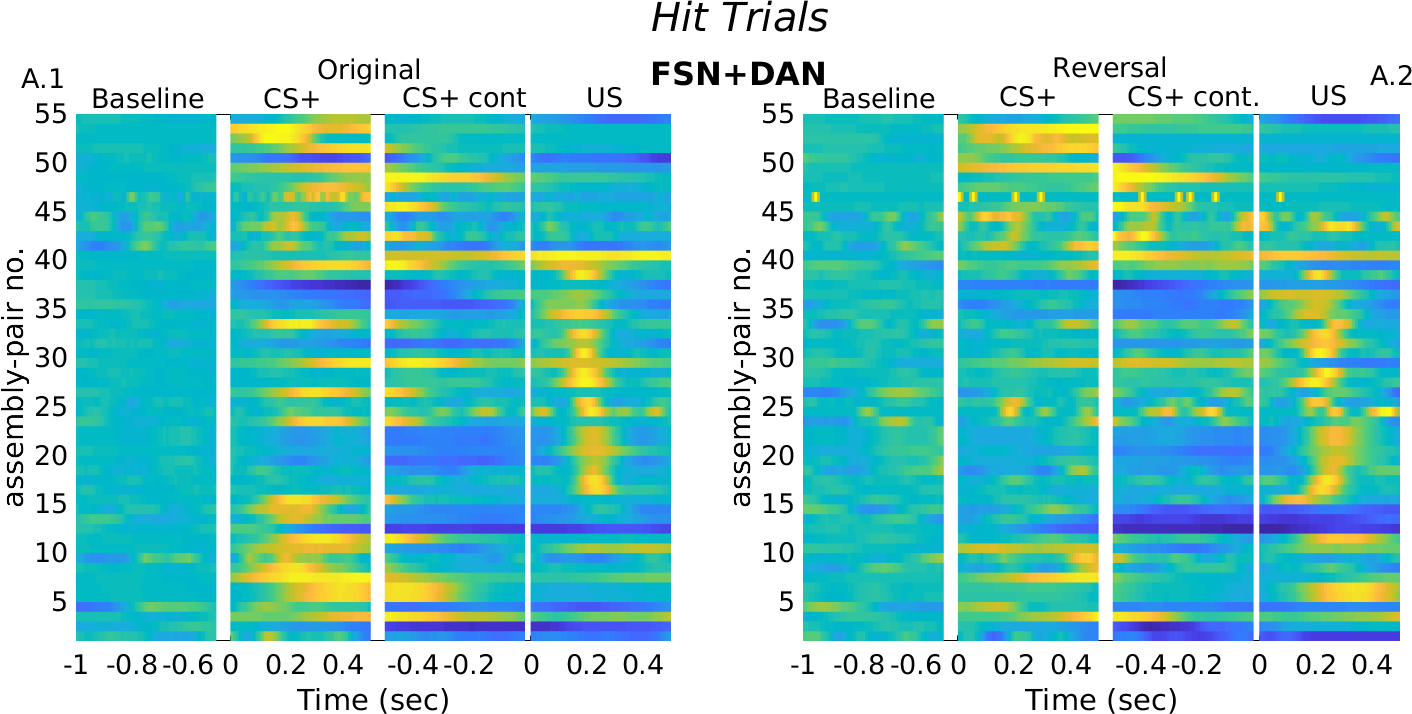
\includegraphics[scale=0.4]{figures/HeatFSN_DANHit1.png} 
 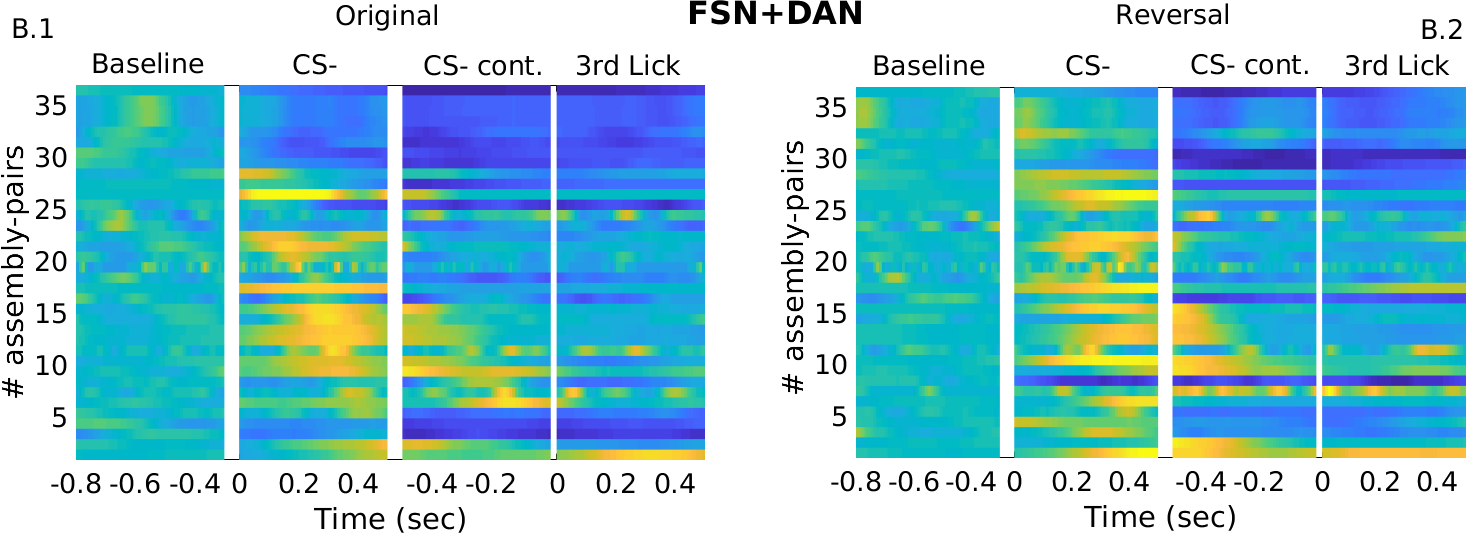
\includegraphics[scale=0.4]{figures/HeatFA_FSN_DAN.png}
 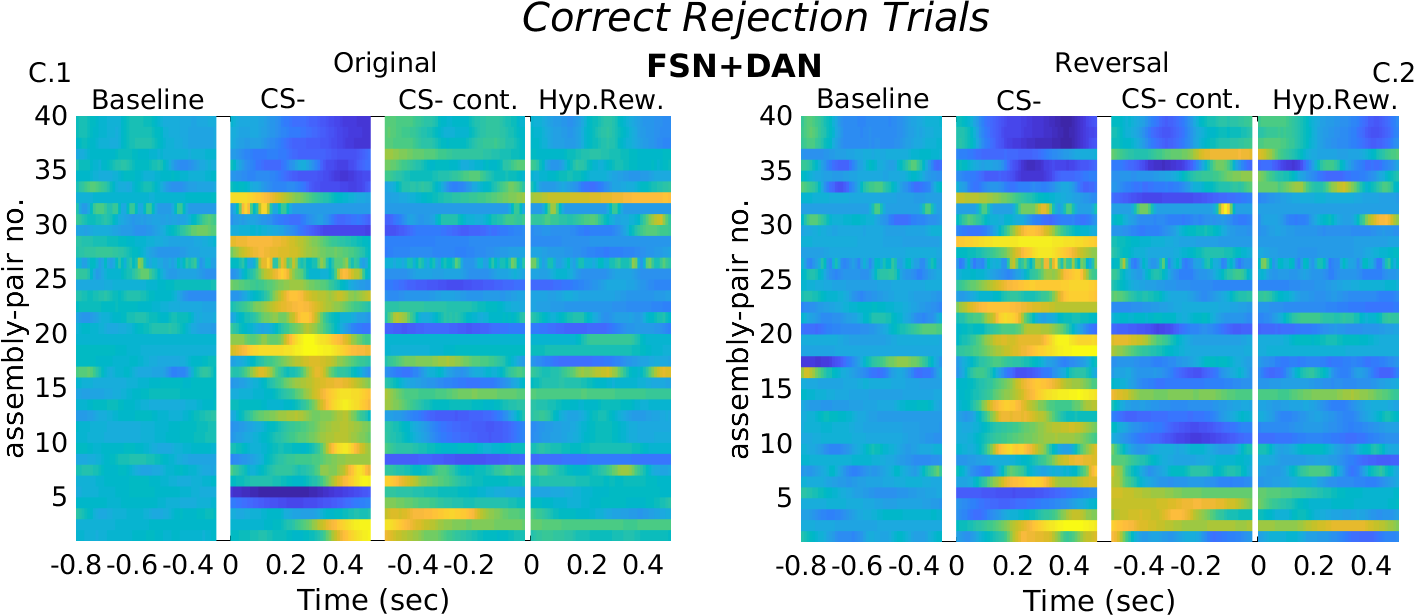
\includegraphics[scale=0.4]{figures/HeatCR_FSN_DAN.png}
  \caption{Heat map of significant activation of FPN-DAN (Friedman test). FSN-DAN assembly-pair activity patterns are diverse in their task dependent activation pattern. In Hit trials (panels A.1, A.2) FSN-DAN show early stimulus responses (CS+) and phasic responses at retrieval (US). In False Alarm trials (panels B.1, B.2) and Correct Rejection trials (boxes C.1, C.2) the activation to the stimulus remained, while no activation in the windows before and after the expected reward time was found.}
  \label{fig:HeatFSN_DANComp}
\end{largefigure}
\section{Conclusion}
In the previous two sections I described the task-related activity of assembly-pair types. I first noticed that different assembly-pairs types showed different task-related patterns of activity, and consequently they could exhibit different coding features.\\The observed activity patterns, at the stimulus presentation and at the retrieval, revealed that VS-VTA pairs were encoding difference between expected and received outcomes.\\In particular from the resemblance of SPN-DAN responses to the rewarded stimulus and expected for prediction error signals, we generated the hypothesis that SPN-DAN assembly-pairs encode prediction signals.\\To prove the aforementioned hypothesis I introduce the learning dynamic in the analysis, through a reinforcement learning model. The prediction signal is considered to be the basis of associative learning (\cite{RescorlaWagner}), with its relation to machine learning algorithms (\cite{SuttonBarto}).\\Despite FSN-DAN pairs seemed to not encode the main component of prediction error, they showed differential activity in Hit, False Alarm and Correct Rejection trials. The unselective and multisensory nature of their response could correspond to a braod range of coding futures, that did not refer to the main component of prediction error, but rather to the detection component, characterized by salience at the stimulus onset, not informative about the specific outcome; as one may expect for VP (\cite{TianHuang} \cite{Berridge}).\\Salience signals are barely explained by the classical reward prediction error signal as parameterized in reinforcement learning model, hence I used FSN-DAN pairs as control in the reinforcement learning model.